\documentclass[english,oneside,color]{htldipl}
% Zulässige Class Options:
%   Hauptsprache: german (default), english
%   Doppelseitig: oneside (default), twoside
%   Syntax-Highlighting: color (default), black

% die folgende Zeile einkommentieren für Arial-Ähnliche Schriftart
%\renewcommand{\familydefault}{\sfdefault}

\graphicspath{{images/}}    % wo liegen die Bilder?

\usepackage{hyperref}
\usepackage{float}
\usepackage{listings}
\usepackage{array}
\usepackage[paper=a4paper,margin=3cm]{geometry}
\usepackage{url}
\usepackage{varioref}
\usepackage{tabularx}
\usepackage{amsmath}
\usepackage{pgfplots}
\usepackage{chngcntr}
\counterwithout{equation}{chapter}

\addbibresource{references}

% uncomment to show subsubsections in toc an number them
% \setcounter{tocdepth}{4}
% \setcounter{secnumdepth}{4}

%%%----------------------------------------------------------
\begin{document}
%%%----------------------------------------------------------

\title{GRAMOC - Gradienten Magnetometer Online Controller}

\abteilung{Informatik}
\schwerpunkt{}
\studienort{Wiener Neustadt}
\schule{HTBLuVA Wiener Neustadt}
\schullogo{htl.jpeg}
\abgabejahr{2017/18}
\betreuerA{Dr. Michael Stifter}
\betreuerB{}
\betreuerC{}
\schuelerA{Nico Kratky}
\evidenzA{5CHIF-13}
\subthemaA{Entwicklung Server, Netzwerkprotokoll}
\schuelerB{Nico Leidenfrost}
\evidenzB{5CHIF-14}
\subthemaB{Entwicklung App, Visualisierung}
\schuelerC{}
\evidenzC{}
\subthemaC{}
\schuelerD{}
\evidenzD{}
\subthemaD{}
\schuelerE{}
\evidenzE{}
\subthemaE{}

%%%----------------------------------------------------------
\frontmatter
\maketitle
\listoftodo\clearpage
\tableofcontents
%%%----------------------------------------------------------

\begingroup
\makeatletter
\newpage
\@twosidefalse
\includepdf[pages=1-1,pagecommand={\chapter[Diplomarbeit Dokumentation]{}}]{images/Formular-printed.pdf}
\includepdf[pages=2-2,pagecommand={\thispagestyle{plain}}]{images/Formular-printed.pdf}
\includepdf[pages=3-3,pagecommand={\chapter[Diploma Thesis Documentation]{}}]{images/Formular-printed.pdf}
\includepdf[pages=4-4,pagecommand={\thispagestyle{plain}}]{images/Formular-printed.pdf}
\endgroup

\chapter{Kurzfassung}
\begin{german}

Diese Diplomarbeit stellt GRAMOC vor. GRAMOC ist ein System, dass es ermöglicht Stahlbänder, ohne die Produktion stoppen zu müssen, effektiv zu charakterisieren. Dies wird durch die Erfindung eines hochsensitiven MEMS Gradienten Magnetometer ermöglicht.

Diese Prozedur steigert nicht nur die Produktivität, sondern ist auch material- und kosteneffizient.

Die ersten Versuche diese Problemstellung zu lösen wurden mit einem TCP-basiertem Server und einer nativen Android Applikation unternommen. Schnell stellte sich heraus, dass dies nicht die geforderten Echtzeitkriterien erfüllen kann. Diese Erfahrung resultierte in einem Neustart des Projektes mit geänderten Anforderungen. Die Android App wurde durch eine Webanwendung mit responsiven Design ersetzt. Dies erweitert nicht nur die Anzahl der unterstützen Endgeräte, sondern bringt auch Vorteile in punkto Drittanbieter Visualisierungsbibliotheken.

GRAMOC besteht letztendlich aus zwei Kommandozeilenprogrammen und einer Web Applikation. Das erste Kommandozeilenprogramm ist der Server, der die vom Sensor empfangenen Daten vorverarbeitet. Dieses Programm führt auch eine dynamische Datenanalyse durch. Das zweite Kommandozeilenprogramm kümmert sich um die Datenspeicherung, da alle Sensordaten in HDF5 Dateien gespeichert werden müssen, um eine nachträgliche Inspektion der Daten zu ermöglichen. Beide Programme laufen auf einem Raspberry Pi 3 Model B. Das Client Programm ist eine Web Anwendung die dazu dient, Sensordaten visuell darzustellen. Auch wird ein Formular zur Verfügung gestellt, um historische Sensordaten aus den HDF5 Datein abfragen zu können. Die kabellose Übertragung von Daten erfolgt über ein Wireless LAN Netzwerk, unterstützt durch ein eigens entwickeltes UDP-basiertes Netzwerkprotokoll.

Die empfangenen Sensordaten werden mittels multipler Linear Regression analysiert. Dies ermöglicht es, mechanische Parameter des Stahlbandes von den magnetischen Daten abzuleiten.

\end{german}

\chapter{Abstract}


% \chapter[Logo]{}
% \vspace*{\fill}
% \begin{center}
% 	\makebox[\textwidth]{
\includegraphics[width=0.6\paperwidth]{gramoc-icon}}
% \end{center}
% \vspace*{\fill}
% \clearpage

%%%----------------------------------------------------------
\mainmatter           %Hauptteil (ab hier arab. Seitenzahlen)
%%%----------------------------------------------------------

\chapter{Introduction}
\label{ch:Introduction}

% what are we trying to solve / what is the problem?
% why is it important?

% minimize faulty material
% change contact pressure of steel belt rolls if something's going wrong
% cost reduction
% automatization (IoT, Industry 4.0)

% perform quality checks with sensors
% mechanical parameters can be calculated from magnetic field data
% highly sensitive MEMS gradient magnetometer
% try to predict faulty material in real time

Industry is ever-changing. Especially people working in the information technology branch know that, since these are the people that have to upgrade the current systems using latest technology. The latest industry-changing milestone was the rise of the so-called Industry 4.0, which combines regular mechanical processes with modern information and communication technology.

Industry 4.0 is a term that was coined by the German government \autocite{Industrie4.0Paper}. It describes the fourth industrial revolution. As explained in \citetitle{Industrie4.0History}, the first industrial revolution took place around 1800 with the rise of steam and water-powered machines \autocite{Industrie4.0History}. One century later electricity heralded the start of the second industrial revolution, production lines being one of the biggest milestones. Also division of labour was first practiced. The third industrial revolution occurred with the invention of computers, robots and computer automation. The fourth and final one basically just refines the third revolution. This revolution includes the term \textit{cyber-physical systems}, which are systems that are controlled by computers, algorithms and sensors. This also means that there has to be some kind of communication between these systems which happens mostly over the internet. Figure \vref{fig:industry40} depicts this sequence of revolutions.

\begin{figure}[H]
    \centering
    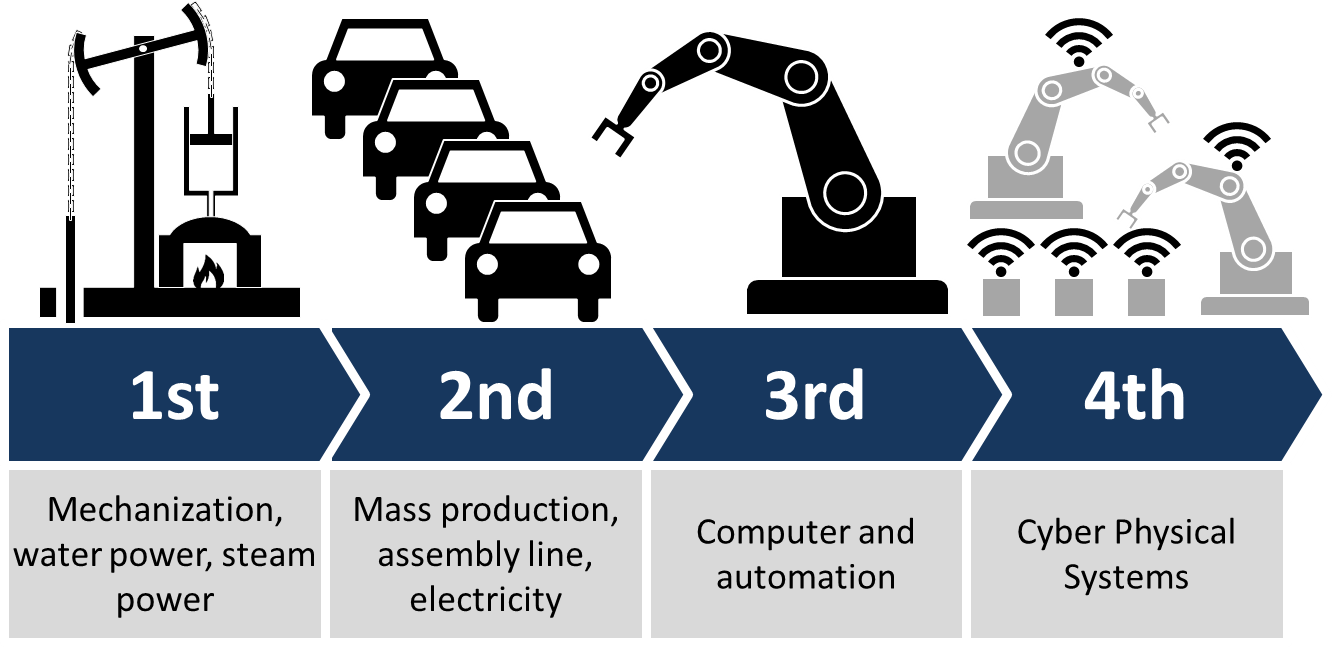
\includegraphics[width=11cm,keepaspectratio]{industry40}
    \caption[The four industrial revolutions that took place over the last centuries]{The four industrial revolutions that took place over the last centuries \autocite{img:industry4.0}}
    \label{fig:industry40}
\end{figure}

This drastic change means that many companies have to adapt to keep up with the competing companies that already have these technologies. Steel belt production companies are no exception. With the invention of a gradient magnetometer that can effectively characterise steel belts, the foundation for this diploma thesis was laid.

\section{Task}

The task of this diploma thesis is to develop a system to read sensor data, process it and visualise the results. Sensor data is continuously read from a highly sensitive MEMS gradient magnetometer. This data is structured as raw binary data and has to be processed by the system. The processed data will also undergo statistical analysis to predict parameters on the basis of this data. After this processing step the data has to be sent wirelessly to a mobile app. This mobile app acts as the client-side of the system. The app visualises the sensor data and its predicted parameters. The app should also offer a way of browsing through historical data that was saved prior.

\subsection{Requirements of GRAMOC}

Server side requirements:

\begin{itemize}
    \item Read data from a sensor
    \item Save sensor data for further inspection
    \item Predict mechanical parameters from sensor data
    \item Send data to clients
    \item Provide historical data to clients
\end{itemize}

Client side requirements:

\begin{itemize}
    \item Visualise sensor data
    \item Provide a form for requesting historical data
    \item Visualise historical data
\end{itemize}

\section{Existing Solutions}

\subsection{Steel Belt Quality Inspection}

Currently there are no solutions for dynamic steel belt characterisation. All these measurements have to be made manually.

The current procedure to inspect the quality of a steel belt is as follows: The first thing that has to be done is to produce a roll of steel belt. To get the quality level of this product, a sample has to be taken from it. There are two samples taken from each steel belt roll, one from the start and one from the end. These two samples can now undergo quality inspection procedures. The results from these tests can be used to assess the produced steel belt. According to these tests, the parameters of the production machines can be adjusted.

This procedure has a few major disadvantages. Firstly, if the product does not pass the quality tests, the whole steel belt has to be discarded. Time and personnel are also two big disadvantages. These quality tests are not only time consuming but they also require special trained staff for conducting these inspections.

\subsection{Handling Sensor Data}

Currently there are a lot of solutions available that can plot sensor data. The majority of these are even free. The one constraint that most of these solutions share is that the sensor has to be directly connected to the computer. As the sensor that is used for this project sends its data over the network, almost all solutions are considered irrelevant. Also some custom features are wanted that these programs do not offer. For example visualizing historical data.

\subsection{Plotting Real Time Data}

\author{Nico Leidenfrost}
%
As already mentioned there are a lot of solutions out there that can be used to plot sensor data. But the one thing that these solutions mostly can not provide is real time plotting. Static plots can be achieved in many different ways, with big amounts of data or just small amounts, many plots combined or divided in separate plots and many more variations are within the bounds of possibility. A lot of these solutions promote themselves with \textit{dynamic data updates} or \textit{streaming data}. That just means that the data can be changed at runtime and therefore some could say the data is displayed in real time. But real time can be defined very differently. As one would say real time applications can update their data once every second, others consider that the data must be updated within less than 20 milliseconds to achieve a high framerate. Most of the solutions available can handle the former definition of real-time but nearly none of them can provide enough performance for the latter. Another important point is the amount of data that one wants to depict, because most of the already existing programs that can handle real-time are just powerful enough to handle small amounts of data.

\section{Outline}

This diploma thesis is structured into two big parts. These parts can be seen as two phases of implementation. Each phase is completely separate. The first phase is a more experimental one as both authors were unfamiliar with these types of projects, so some experience had to be made. At the end of this phase there was a big cut and the project was restarted from the beginning. The second phase discusses the different approaches and decisions that were made starting from this cut. The second phase was not only better planned, but the decisions that were made, were mostly made out of experience from the first phase.

% \chapter{Project Management}
\label{ch:Project Management}
There are various projects no matter if it's developing software or even building a bridge, each of them needs to be managed carefully because otherwise it could end with a low quality outcome, time delays or even with enormous costs that the ones running the project can not handle. To prevent all these horrible scenarios project management helps with the application of knowledge, skills, tools and techniques. Project management as it's used and performed nowadays exists since the mid-20th century, but earlier, much simpler versions of it were used since ever.

\section{Kanban}

\subsection{Description of Kanban}
Kanban is a technique to manage software development in a project. It utilizes the just-in-time (JIT) production system and easily reveals possible bottlenecks in the software development pipeline. Kanban provides information in a visual way instead of a textual, therefore the brain can extract information much quicker. The reason is that the human brain is able to processes visual information 60 000 times faster than text \cite{WhatIsKanban}. Kanban uses sticky notes or some sort of cards on a board to display the information. This method packs the pure text information in a bigger picture that the brain can now process faster.

\subsection{How Kanban works}
Kanban has four core principles \cite{WhatIsKanban}.
\begin{enumerate}
    \item \textbf{Visualize Work}

    By visualizing the work and workflow in a project, it's easier to observe the flow of work through the whole Kanban system. Also problems like bottlenecks, blockers and queues can be spotted immediately.

    \item \textbf{Limit Work in Process}

    Kanban limits the amount of unfinished work in process. By doing so it reduces the time one item needs to travel through the Kanban system. That brings the advantage of less task switching and constantly reprioritizing.

    \item \textbf{Focus on Flow}

    By implementing work-in-progress (WIP) limits and team-driven policies the Kanban system can be optimized to improve the workflow. With its methods the flow can be analyzed and it can indicate possible future problems.

    \item \textbf{Continuous Improvement}

    Once the Kanban system is established, teams can track their efficiency by measuring flow, quality and throughput of work items they are assigned to. This can help a team a lot to improve and take their efficiency to a higher level.
\end{enumerate}

\subsection{History of Kanban}
Kanban was developed by Toyota in the late 1940s, the idea of Kanban came up from an unlikely source, the supermarket. They realized that the workers there ordered their goods if the stock was going near zero instead of order more goods if they are available at a vendor. So they ordered their goods after a ``just-in-time'' system. Kanban is Japanese for ``sign'' or ``signboard'', so Toyota invented a system that allowed teams to communicate better and showed them what work is needed to be done and when it's needed \cite{WhatIsKanban}.

\section{Scrum}

\subsection{Description of Scrum}
Scrum is a process framework to control and manage complex software development projects, it reduces the complexity of the whole system and focuses on a product that meets the business needs. ``Scrum makes clear the relative efficacy of your product management and development practices so that you can improve.'' \cite{ScrumGuide}

\subsection{How Scrum works}
Scrum consists of a number of entities that include \cite{WhatIsScrum}:
\begin{itemize}
    \item \textbf{The Scrum Values} originally weren't included in the official Scrum guide, but due to most people considered them as a part of Scrum they were added in July 2016. These values are Commitment, Courage, Focus, Openness and Respect.

    \item \textbf{The Scrum Roles} are three roles every Scrum team needs to consist of. There is the ``Product Owner'', who needs to manage the Product Backlog. He needs to make sure the items are clearly expressed and in an order so that the team can achieve the best possible result. Theres also the ``Scrum Master'', who makes sure Scrum is used and understood properly. He also tells people outside of the Scrum team how they should interact with the team to maximize the output of the team. All of the other members in the Team are part of the ``Development Team''. Such a team is self-organized, cross-functional and there is no particular ranking in the team which means everybody is on the same level. The Development Team and only the Development Team is responsible to complete tasks from the Product Backlog at the end of each Sprint.

    \item \textbf{The Scrum Events} are used to create a regularity and minimize the effort of meetings outside the Scrum meetings. These events all have a fixed timespan and can't be shortened or lengthened. The Events embedded in Scrum are:
    \begin{enumerate}
        \item \textbf{Sprint}

        Each Sprint has a predefined timespan up to one month, in this period of time the Development Team should create a releasable increment to the product. During the Sprint, nobody should make changes that would compromise the goal of the Sprint, also the stated quality of the product does not decrease. The scope of a Sprint can be clarified and re-negotiated with the Product Owner during the Sprint, when a Sprint finishes the next Sprint starts immediately.

        \item \textbf{Sprint Planning}

        The Sprint Planning Event takes place before each Sprint, in this meeting items from the Product Backlog are moved into the Sprint Backlog. These items do not have to be finished in one Sprint as a Sprint is defined by its time limit and not by the items in the Sprint Backlog.

        \item \textbf{Daily Scrum}

        In the Daily Scrum meeting the Development Team creates a plan for the next 24 hours. To do so the attendees analyze the work that has been done so far and with this knowledge they determine what to do until the next meeting. This meeting has a duration of at most 15 minutes and takes place every day in the same place at the same time.

        \item \textbf{Sprint Review}

        This meeting is held at the end of each Sprint, its purpose is to analyze the outcome and what items in the Sprint Backlog were actually finished in this Sprint. Attendees of this meeting are the Scrum team and the stakeholders, both groups should collaborate on the next things that could be done.

        \item \textbf{Sprint Retrospective}

        The main focus in this particular meeting lays on the improvement that can be done during the next Sprint. The topics discussed in the Sprint Retrospective are ``What went well in the Sprint'', ``What could be improved'' and ``What will we commit to improve in the next Sprint''.
    \end{enumerate}

    \item \textbf{Scrum Artifacts} represent the work that is to do or already is done to make it easier to inspect and adapt the particular work units. Therefore there are three Artifacts, the first one is the \emph{Product Backlog}, here defined are requirements that might be needed in the product. The Product Backlog evolves with the product itself, there will be requirements added and removed based on the results of the Sprints finished. The second Artifact is the \emph{Sprint Backlog}, in here are items that are assigned to do in the corresponding Sprint plus a plan how to accomplish the Sprint goal. The last Artifact is the \emph{Increment}, this is described as the sum of all items in the Product Backlog that are finished within the Sprint.
\end{itemize}

\section{Scrumban}

\subsection{Description of Scrumban}
The term ``Scrumban'' is a composition of the two terms ``Scrum'' and ``Kanban'', therefore Scrumban is a project management technique mix of Scrum and Kanban. Scrumban takes the best of both management systems and combines them into one powerful tool to help teams develop their products even faster than before.

\subsection{How Scrumban works}
Scrum is based on fixed time windows called Sprints and the communication between the people delivering the product, Kanban however is based on fixed pieces of work and showing when they need to be done. So Scrumban takes the workpiece based Kanban system and adds the communicational aspects of scrum.

\subsection{Application of Scrumban in this Project}
Scrumban was chosen to be applied in this project because it fitted the already used project management methods. With this technique the tasks could be finished even faster than before and even with a higher quality result. There were meetings as defined within Scrum and a couple of Kanban-boards assigned to the proper members of the team.


\chapter{Real Time Systems}
\label{ch:realtimesystems}

\author{Nico Kratky}
%
\section{Definition}

Real-time systems (RTS) have one big constraint that normal computer programs don't have, time. Contrary to normal applications, where the correctness of data only depends on the made computations, RTS also depend on the timing of these computations. This time limit, that has to be adhered to, is also often called deadline.
Types of RTS are mostly differentiated between what happens when the deadline is not met. There are three basic types of real-time systems.

\subsection{Hard Real-time Systems}

In hard real-time systems an overrun in response time will lead to failure \autocite{RealTimeHermannKopetz}. This can mean big financial losses of even danger to life. An example for a hard RTS would be the ECU (Electronic Control Unit) of a modern car. If the timing of the fuel injection or ignition is not correct, the engine could fail and lead to a crash. Another example would be the control unit for airbags. This unit has to constantly monitor the cars crash sensors and decide whether to trigger the airbags or not. This system would have to fulfill the hard criteria because if the airbags trigger to late, then human safety can not be guaranteed.

\subsection{Soft Real-time systems}

A soft real-time system still does have a deadline but it is not that big of a deal if it is not met \autocite{RealTimeHermannKopetz}. There are some consequences to not meeting the time limit but they are tolerable. A video-stream is a example for a soft real-time system. If some frames are not delivered in time the video will stutter, but the content will still be delivered.

\subsection{Firm Real-time systems}

In firm real-time systems the data will be useless if the time limit is overrun \autocite{RealTimeHermannKopetz}. The data will then be discarded. This is the type of RTS that GRAMOC can be associated with.

\author{Nico Leidenfrost}
%
\section{Programming Language}
In the early days of computer programming, there were only a few programming languages available. Today there is a broad variety of them ready to be used. The popularity of a language can reach from only a few users to worldwide professional use. To create applications that are able to process streaming data in real-time, only a minority of languages are considered useful. Reasons why some programming languages are used more often than others are \autocite{RealTimeByronEllis}:

\begin{itemize}
    \item The high performance of the native implementation
    \item The ease of use
    \item The popularity and community support
\end{itemize}

\subsection{Java}
Java was a long time a major language for developing real-time web applications because of their ``Write once Run everywhere'' principle. Thats possible because of the Java Virtual Machine(JVM), all the code written in Java is compiled to run inside this virtual machine, therefore every system that can run the JVM, can also run the same Java code as all the other systems. The client side development was early replaced by Adobe's Flash project, since then Java is disabled per default in most of the web browsers.

But Java did find its place at the server side, the so called back-end, especially because the Java Database Connectivity(JDBC) was developed in the early stages of Java and enabled an easy way to interact with databases. One of the most crucial points in why somebody would use Java was because it was easy to integrate third-party packages as a result of many available package management systems, but also the deployment of the finished application was easier than the deployment of an application from their main competitor C++.

\subsubsection{Scala and Clojure}
A variety of languages were designed to also run inside the JVM, two of the more popular ones in real-time programming are Scala and Clojure. Both these languages can use Java packages as they run in the same environment. Scala is mostly used for academic projects, but as of their rich standard library it is also used in high performance server applications. The distinction to Java is that Scala utilises features from functional programming languages although it is declared as a object-oriented language. Clojure is a dialect of Lisp that can also make use of Java packages.

\subsection{JavaScript}
JavaScript is the most popular programming language in terms of web development, it is supported by every browser and during the development every browser developer wanted to have the fastest JavaScript engine. Thanks to that JavaScript is now incredibly fast and capable of implementing web applications on its own. The only similarities between JavaScript and Java are the name, which was a marketing gag and the syntax, because they both inherit some parts of it from C/C++, all other aspects of these two languages are distinct from each other. JavaScript is a functional programming language which means functions are treated the same way as data. In JavaScript a function can be assigned to a variable and be passed to another function, a lot of JavaScript frameworks and libraries rely on that feature. Since JavaScript quickly gained a lot popularity in the front-end development it is also capable of running in the back-end, most of the time as a Node.js server (see section \vref{sec:nodejs}).

\subsection{C/C++}
These two languages are known for their efficiency and therefore are often considered to be used within real-time projects. C is widely used in embedded system programming while C++ is used in all kinds of programming. C++ is a superset of C, regardless of that fact C is still used in low-level system programming because of the simplicity. C++ is more complex than C but it also offers features from object-oriented programming. C as well as C++ were first introduced way before the other languages mentioned here, therefore the developers had enough time to optimise the compilers for these languages, which resulted in very efficient code at runtime. Since these languages are considered as low-level programming languages a developer can gain control over system resources more easily and use them efficiently, but this can also be seen as a huge problem when used by people that do not have the required skills to use it correctly or people how exploit this feature on purpose. High performance applications like video games, as well as real-time applications rely heavily on C++ because of its performance.

\subsection{Go}
Go is a language developed at Google based on the C language but with mechanisms included that provide concurrency. This language is still under development and therefore the variety of available libraries and community support is not as great as with the other languages, but its benchmark performance on web server development is still very good.

\section{Data Transfer}
In order to build a application that is capable of displaying sensor data in real-time like GRAMOC it is crucial to find the optimal way to transfer data from the server to the client. There are a lot of solutions to this problem, but two of them are especially popular when it comes to real-time communication:

\begin{itemize}
    \item Sever Sent Events
    \item WebSockets
\end{itemize}

\subsection{Server Sent Events}
\label{subsec:sse}
Server Sent Events(SSE) were introduced in 2006 as a protocol to push data from a server to a client \autocite{sse}. Before SSE was introduced many client server communications relied on polling, a technique where the server was asked for new information by the client in a constant interval. This technique obviously created an enormous amount of overhead, because every time a request for new data was send there had to be a new HTTP connection to be established and afterwards destroyed. SSE was build to be efficient, it only creates one HTTP connection where all the data from the server is pushed and then received by the client through events. The biggest advantage of SSE is of course the long lived connection between the server and the client, but there are also a few downsides of this protocol. The main problem is that the communication is unidirectional, which means the client can receive data from the server, but can not send any data back. Since GRAMOC relies on bidirectional communication between client and server this method is unqualified to be used in this project. A few use cases of SSE would be notifications, status updates or the streaming of stock tickers.

\subsection{WebSockets}
In 2011 the WebSocket protocol was standardised by the RFC6455 \autocite{rfc6455}. WebSockets offer instead of unidirectional communication like server sent events, bidirectional communication between server and client (see subsection \vref{subsec:sse}). WebSockets communicate per default over port 80, therefore there are no problems with the firewall, but unlike the protocols before they perform a handshake on connection to upgrade the connection. The WebSocket protocol is way more complicated than the SSE protocol, but at the time of writing most browsers offer solid native WebSocket support and a lot of libraries that implement WebSockets are existing and well maintained. The probably most popular WebSocket library is called socket.io, this library is also used within GRAMOC to communicate between the server and the client (see section \vref{sec:socketio}). Other use cases of WebSockets would be applications that rely on bidirectional real-time updates like games or chat applications.


\part{Implementation Phase 1}
\chapter{Networking Technologies}
\label{ch:networkingtechnologies}

\author{Nico Kratky}
%
\section{Networking in GRAMOC}

Because GRAMOC is based on basic a client-server architecture, a common way of communication had to be developed. This development process resulted in GSDEP.

\section{GSDEP}

GRAMOC Sensor Data Exchange Protocol (GSDEP) is GRAMOC's Network Protocol that is used for sending large amounts of sensor data to the clients. It is built on top of the TCP/IP stack \cite{rfc793, rfc791}.

\subsection{Data Flow}
\label{sec:networking_data-flow}

Figure \ref{fig:handshake} depicts the handshake performed by GSDEP that is based on TCP's three-way handshake. The Client sends a synchronize (SYN) message to the server to let it know that it wants to connect. If the server can accept new Clients it returns an acknowledgment message (ACK). The client then also returns this acknowledgment message to inform the server that it is indeed connected. The connection now is established.

\begin{figure}[H]
    \centering
    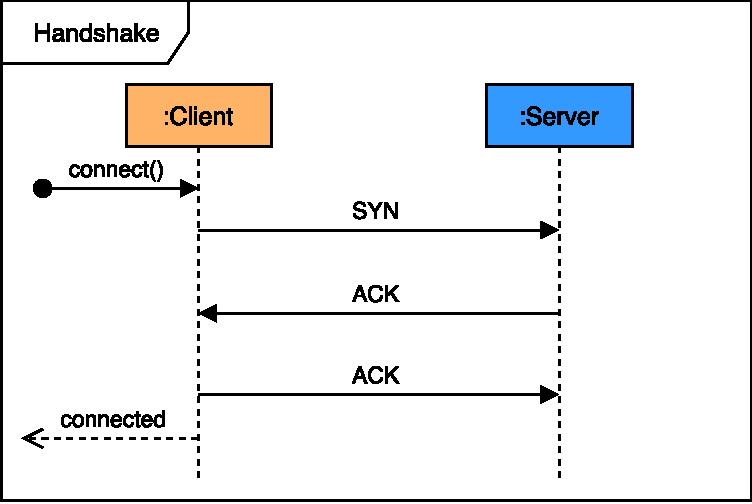
\includegraphics[width=8cm,keepaspectratio]{gsdep_handshake}
    \caption{TCP-like three way handshake performed on client connect}
    \label{fig:handshake}
\end{figure}

If a client wants to disconnect from the server it will send a disconnect message (FIN) to the server. Before it actually disconnects, it has to wait for the server to finish cleaning up and return the FIN packet. After the client has received this message, it can close the connection and shut down. This procedure is shown in Figure \ref{fig:disconnect}.

\begin{figure}[H]
    \centering
    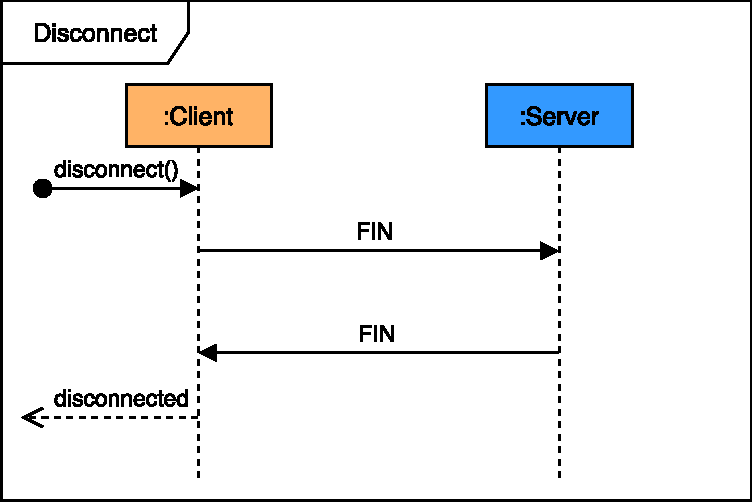
\includegraphics[width=8cm,keepaspectratio]{gsdep_disconnect}
    \caption{Two way handshake performed on client disconnect}
    \label{fig:disconnect}
\end{figure}

\subsection{Data Interchange Format}

Every message is made up of a header and the actual payload that will be transmitted. The header includes additional information that is used by the receiving end to determine the size of the payload (see \ref{sec:messageframing}), to differentiate between different kinds of messages (see \ref{sec:channels}) and to rebuild the message data to its correct data type. As depicted in Figure \ref{fig:packet}, the header consists of 4 bytes message length and 2 bytes each for data type and channel.

\begin{figure}[H]
    \centering
    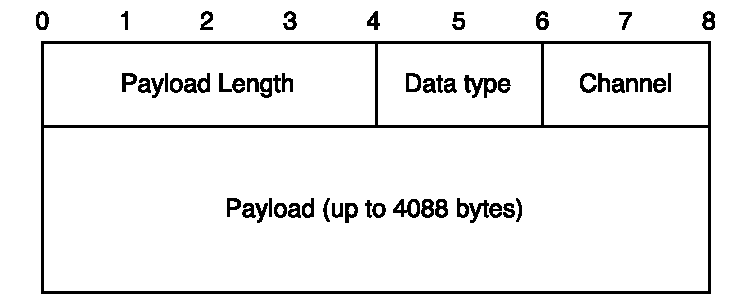
\includegraphics[width=8cm,keepaspectratio]{gsdep_packet}
    \caption{Structure of one packet sent by GSDEP}
    \label{fig:packet}
\end{figure}

\subsection{Commands}
\label{sec:networking_command}

Commands are special messages that require further action to be taken. These commands can either be used during the connect or disconnect handshakes, or to request data.

\begin{table}[H]
    \centering
    \begin{tabular}{| l | l | p{5cm} |}
    \hline
    \textbf{Command} & \textbf{Used by} & \textbf{Meaning} \\ \hline
    SYN & client & Tells the server that a new client is waiting for the connection procedure \\ \hline
    ACK & server \& client & Tells the other end that it acknowledges the previous command \\ \hline
    FIN & server \& client & Tells the other end that it will disconnect \\ \hline
    STD & client & Tells the server that a client requests data\\ \hline
    SPD & client & Tells the server that a client does not want any more data\\
    \hline
    \end{tabular}
    \caption{Commands sent by one of the connection partners and what they do}
    \label{tab:commands}
\end{table}

\subsection{Channels}
\label{sec:channels}

In the case of GRAMOC, where large amounts of data are received in short periods of time, it is crucial to differentiate between communication data and sensor data in split seconds. To accomplish this a 2 byte unsigned short is included in the packet header. This information can the be used to tell apart these two types of data.

\begin{table}[H]
    \centering
    \begin{tabular}{| l | c |}
    \hline
    \textbf{Channel} & \textbf{Value} \\ \hline
    Communication & 1 \\ \hline
    Data & 2 \\
    \hline
    \end{tabular}
    \caption{Channels used to distinguish between message types}
    \label{tab:channels}
\end{table}

\subsection{Message framing}
\label{sec:messageframing}
Because TCP operates with streams of data and not packets of data, messages have to be framed so that the receiving end knows what one message is. This can be achieved in two ways. \cite{MessageFramingCleary,MessageFramingSkotzko}

\subsubsection{Length Prefixing}

One method of message framing is to prefix each message with its length. When doing so the format of this prefix has to be stated explicitly. In the case of GSDEP that is a ``4 byte unsigned integer''.

\paragraph{Sending}

First, the message has to be encoded into its binary representation. To send this message, the length followed by the binary encoded message simply has to be sent.

\paragraph{Receiving}

Receiving one message is done by first reading into a buffer with the length of the length prefix (in this instance the buffer would be 4 bytes long). Then the payload is read into a second buffer with the just read length. When this buffer is full, one message has been read.

\subsubsection{Delimiters}

\paragraph{Sending}

Messages can also be framed by using delimiters. This can be done by sending a special character between each message. This character can either be a character that does not show up in actual messages (e.g. a Null character), or a character that is present in a message. If the second approach is used, every message has to be run through an escaping process which replaces these characters in the messages.

\paragraph{Receiving}

Receiving delimited messages is relatively straightforward. One message is read when a delimiter is reached. This message has to be passed to an unescaping function when a delimiter character is chosen that can exist in messages.

\subsubsection{Security Concerns}

Whichever solution is chosen, each solution has to provide code regarding Denial of Service (DoS) attacks. Wether a very big message length or large amounts of data without a delimiter are received, both can result in Out of Memory Exceptions.

\chapter{Server}
\label{ch:server}

\author{Nico Kratky}
%
A server is a computer program that supplies clients with services. The term 'server' often refers to the machine on which the program is running on. In this project the server has to accomplish several tasks. It has to read data from the sensor that is used, and distribute this data to clients. To do this it also has to manage clients and incoming connection requests.

\section{Hardware}
\todo{Put something here}
\subsection{Raspberry Pi 3 Model B}
% The Raspberry Pi is a small single-board computer originally created to teach children how to program \autocite{RasPi}. It was developed by the Raspberry Pi Foundation. There are numerous options for expanding the capabilities of the Raspberry Pi. One being the use of General-purpose input/output (GPIO) pins. They can be used to connect so-called HAT's (Hardware Attached on Top) or Shields (this term evolved from Arduino-land). These add-on boards are mounted to the Raspberry Pi by connecting the GPIO pins to the board and screwing them together. They mostly provide additional hardware to extend the application possibilites and to achieve the desired goal. Further advantages are its relatively small footprint and its low cost. Also, a wide variety of Linux distributions have been adapted to the hardware. Having these advantages was the decisive factor for choosing the Raspberry Pi 3 Model B.\\
% The specifications of the Raspberry Pi 3 Model B are:

The Raspberry Pi is a small single-board computer, developed by the Raspberry Pi Foundation \autocite{RasPi}. Originally it was created to teach children how to use computers and more importantly, how to program them. The biggest advantage of these mini-computers is the variety of extension possibilities. These extension are so-called HAT's (Hardware Attached on Top) or Shields (which is a term that is more often used when talking about Arduinos). They are connected by using the on-board General-purpose input/output (GPIO) pins. They mostly provide additional hardware to extend the application possibilities and to achieve the desired goal. Further advantages are its relatively small footprint, low cost and wide-variety of available Linux distributions. Having these advantages was the decisive factor for choosing the Raspberry Pi. In this project the latest available version, which is the Raspberry Pi 3 Model B, was used. Specifications of this computer are listed in table \vref{tab:raspispec}.

\begin{minipage}{\textwidth}
\begin{table}[h]
    \centering
    \begin{tabularx}{\linewidth}{| l | X |}
    \hline
    \textbf{SoC} & Broadcom BCM2837 \\ \hline
    \textbf{CPU} & 4x ARM Cortex-A53, 1.2GHz \\ \hline
    \textbf{GPU} & Broadcom VideoCore IV \\ \hline
    \textbf{RAM} & 1GB LPDDR2 (900MHz) \\ \hline
    \textbf{Networking} & 10/100 Ethernet, 2.4GHz 802.11n wireless \\ \hline
    \textbf{Bluetooth} & Bluetooth 4.1 Classic, Bluetooth LE \\ \hline
    \textbf{Storage} & microSD \\ \hline
    \textbf{GPIO} & 40-pin header, populated \\ \hline
    \textbf{Ports} & HDMI, 3.5 analogue audio-video jack, 4x USB 2.0, Ethernet, Camera Serial Interface (CSI), Display Serial Interface (DSI) \\ \hline
    \end{tabularx}
    \caption{Raspberry Pi 3 Model B specifications}
    \label{tab:raspispec}
\end{table}
\end{minipage}

\begin{figure}[H]
	\centering
	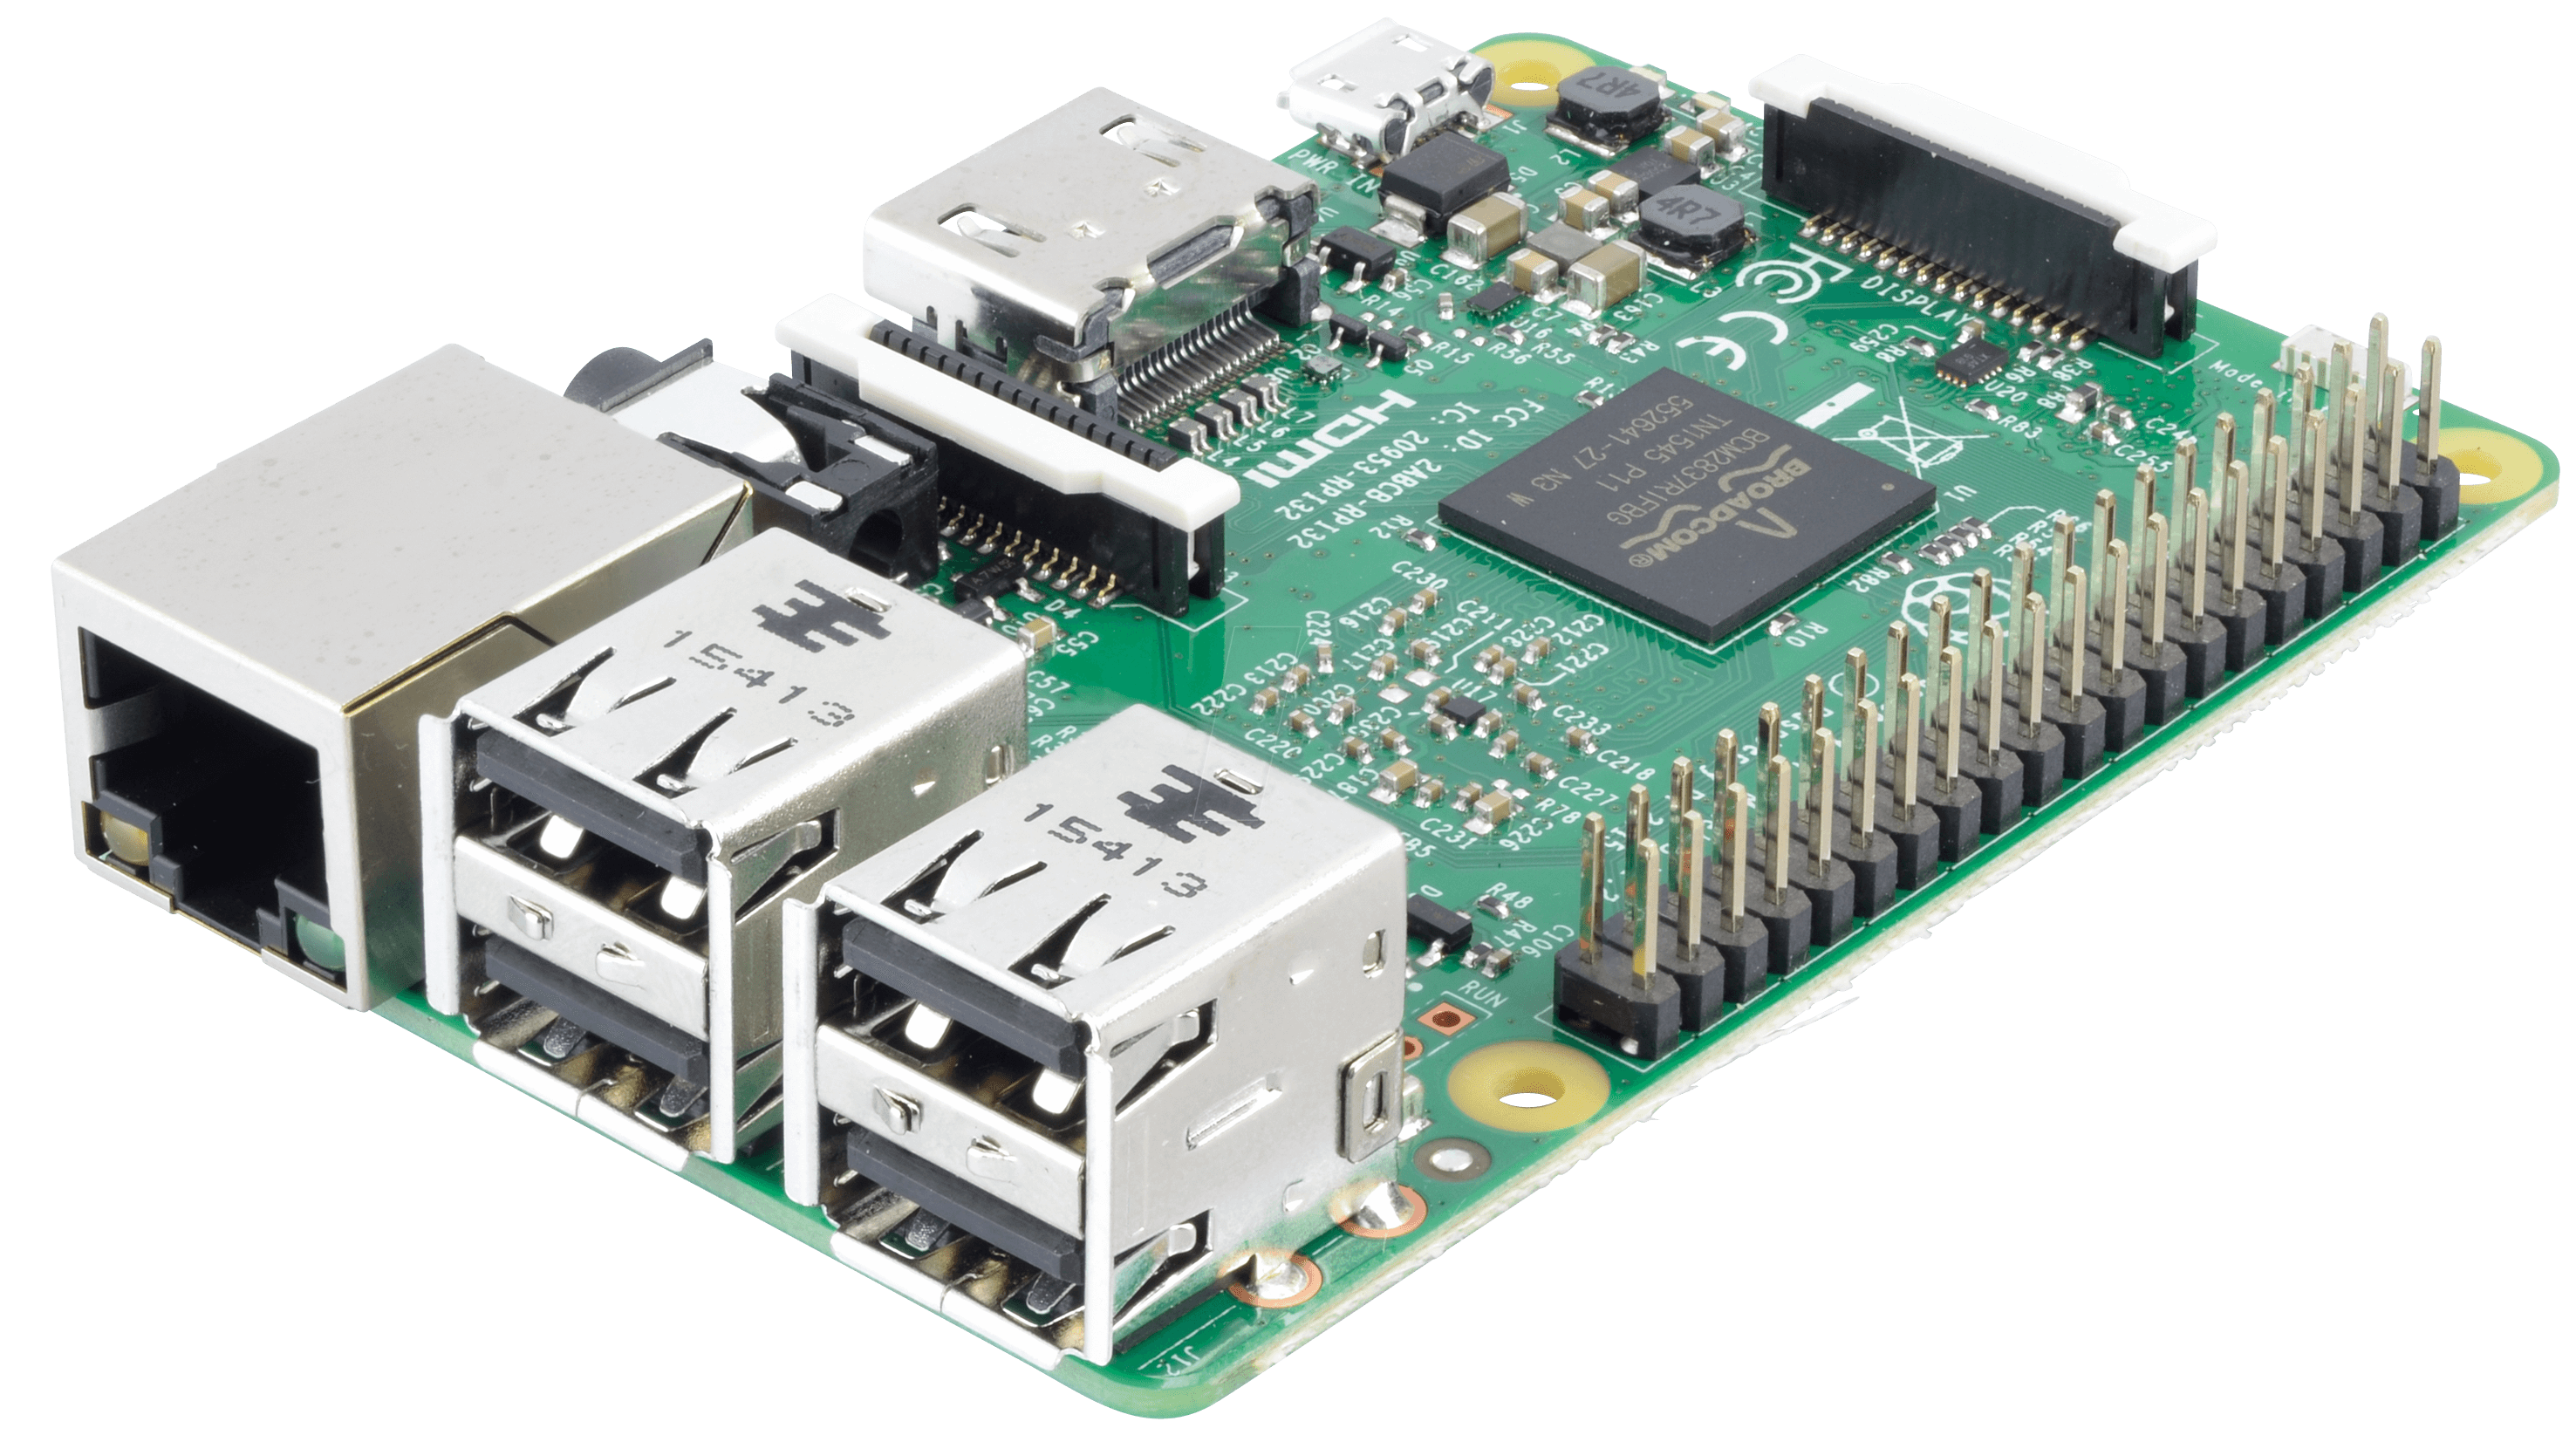
\includegraphics[width=10cm,keepaspectratio]{raspberrypi3b}
	\caption[Raspberry Pi 3 Model B]{Raspberry Pi 3 Model B\footnotemark}
	\label{fig:raspberrypi3b}
\end{figure}

\footnotetext{\cite{img:raspi}}

\subsection{Raspberry Pi SenseHAT}

The SenseHAT was made especially for the Astro Pi mission, where student could create and code projects, which were then run on the International Space Station by astronaut Tim Peake \autocite{AstroPiMission}. This board was chosen because it offers a wide variety of sensors and therefore offers many possibilities in terms of testing GRAMOC. Figure \vref{fig:sensehat} shows a SenseHAT that is not attached to a Raspberry Pi.

The Raspberry Pi Sense HAT includes following sensors and inputs/outputs \autocite{SenseHAT}:

\begin{itemize}
	\item ST LSM9DS1 Inertial measurement sensor
		\begin{itemize}
			\item 3D accelerometer
			\item 3D gyroscope
			\item 3D magnetometer
		\end{itemize}
	\item ST LPS25H barometric pressure and temperature sensor
	\item ST HTS221 relative humidity and temperature sensor
	\item Alps SKRHABE010 5-button mini-joystick
	\item 8x8 RGB LED matrix
\end{itemize}

Although GRAMOCs main task is to charactarize steel belts using a magnetometer, a Raspberry Pi SenseHAT add-on board was used to get sensor data. It was dicided to use the now available accelerometer to perform measurements because it's easier to control the sensor data than by using the magnetometer. Different sensor values can be generated by simply moving around the Raspberry Pi with the attached SenseHAT.

\begin{figure}[H]
	\centering
	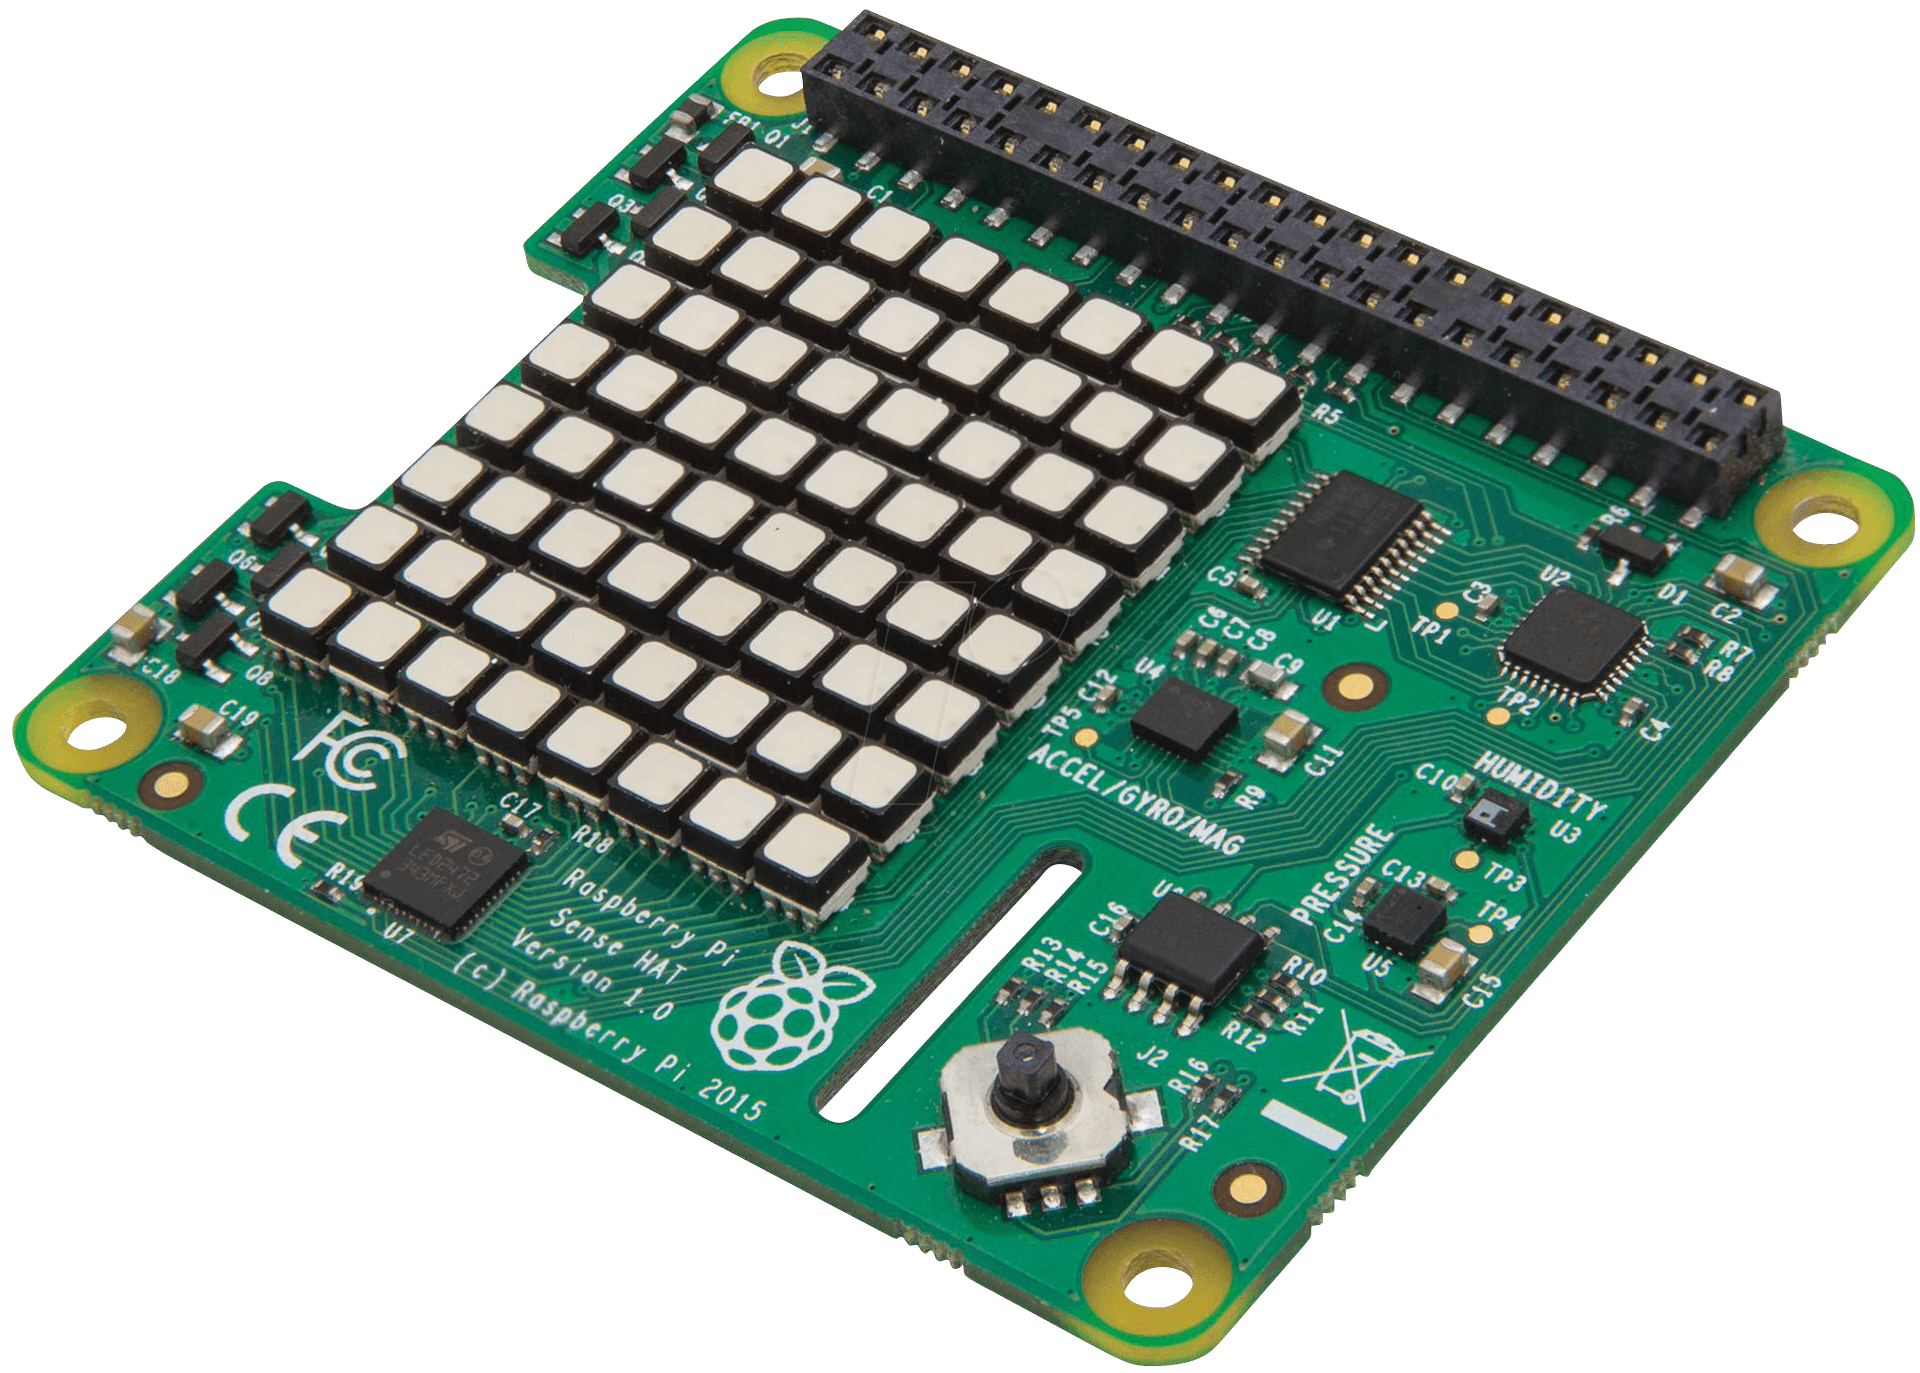
\includegraphics[width=8cm,keepaspectratio]{sensehat}
	\caption[Raspberry Pi SenseHAT]{Raspberry Pi SenseHAT\footnotemark}
	\label{fig:sensehat}
\end{figure}

\footnotetext{\cite{img:sensehat}}

\section{Implementation}

The server program of GRAMOC is completely written in Python. This allows for great compatibility as Python comes preinstalled on many systems.

\subsection{Programming Language}

Python is a simple yet powerful, modern programming language and supports both procedure-oriented as well as object-oriented programming. It was developed by Guido van Rossum at Centrum Wiskunde \& Informatica (CWI) in the Netherlands in 1989 and first released in 1991 \autocite{HistoryOfPython}. It was meant to be a successor to the ABC programming language. Python is a high-level language and therefore includes features such as automatic memory management.

Python is currently available in version 3.6.2. Nevertheless version 2.7 is still available as the Python Software Foundation announced that it will be supportet until 2020, effectivly making it an Long-term support version. Despite that, Python 3.6.2 was chosen for GRAMOC as the Foundation also encourages users to use the newest version if possible. Another reason for choosing the newer version is that GRAMOC does not have to be backwards compatible to any existing software.

\section{Program Flow}

As depicted in figure \vref{fig:server-program-flow}, the server starts accepting new connections right after is has started. It then performs the handshake that is required by GSDEP (further explained in \vref{sec:networking_data-flow}). If this handshake is performed without errors, the server starts listening for data from this now connected client on a separate thread. While this thread is running it receives one message and checks if it is a command (see \vref{sec:networking_command}). If it is, the message is interpreted and the appropriate function is executed. This thread is kept alive until the client disconnects or the server is shutdown by the user.

\begin{figure}[H]
	\centering
	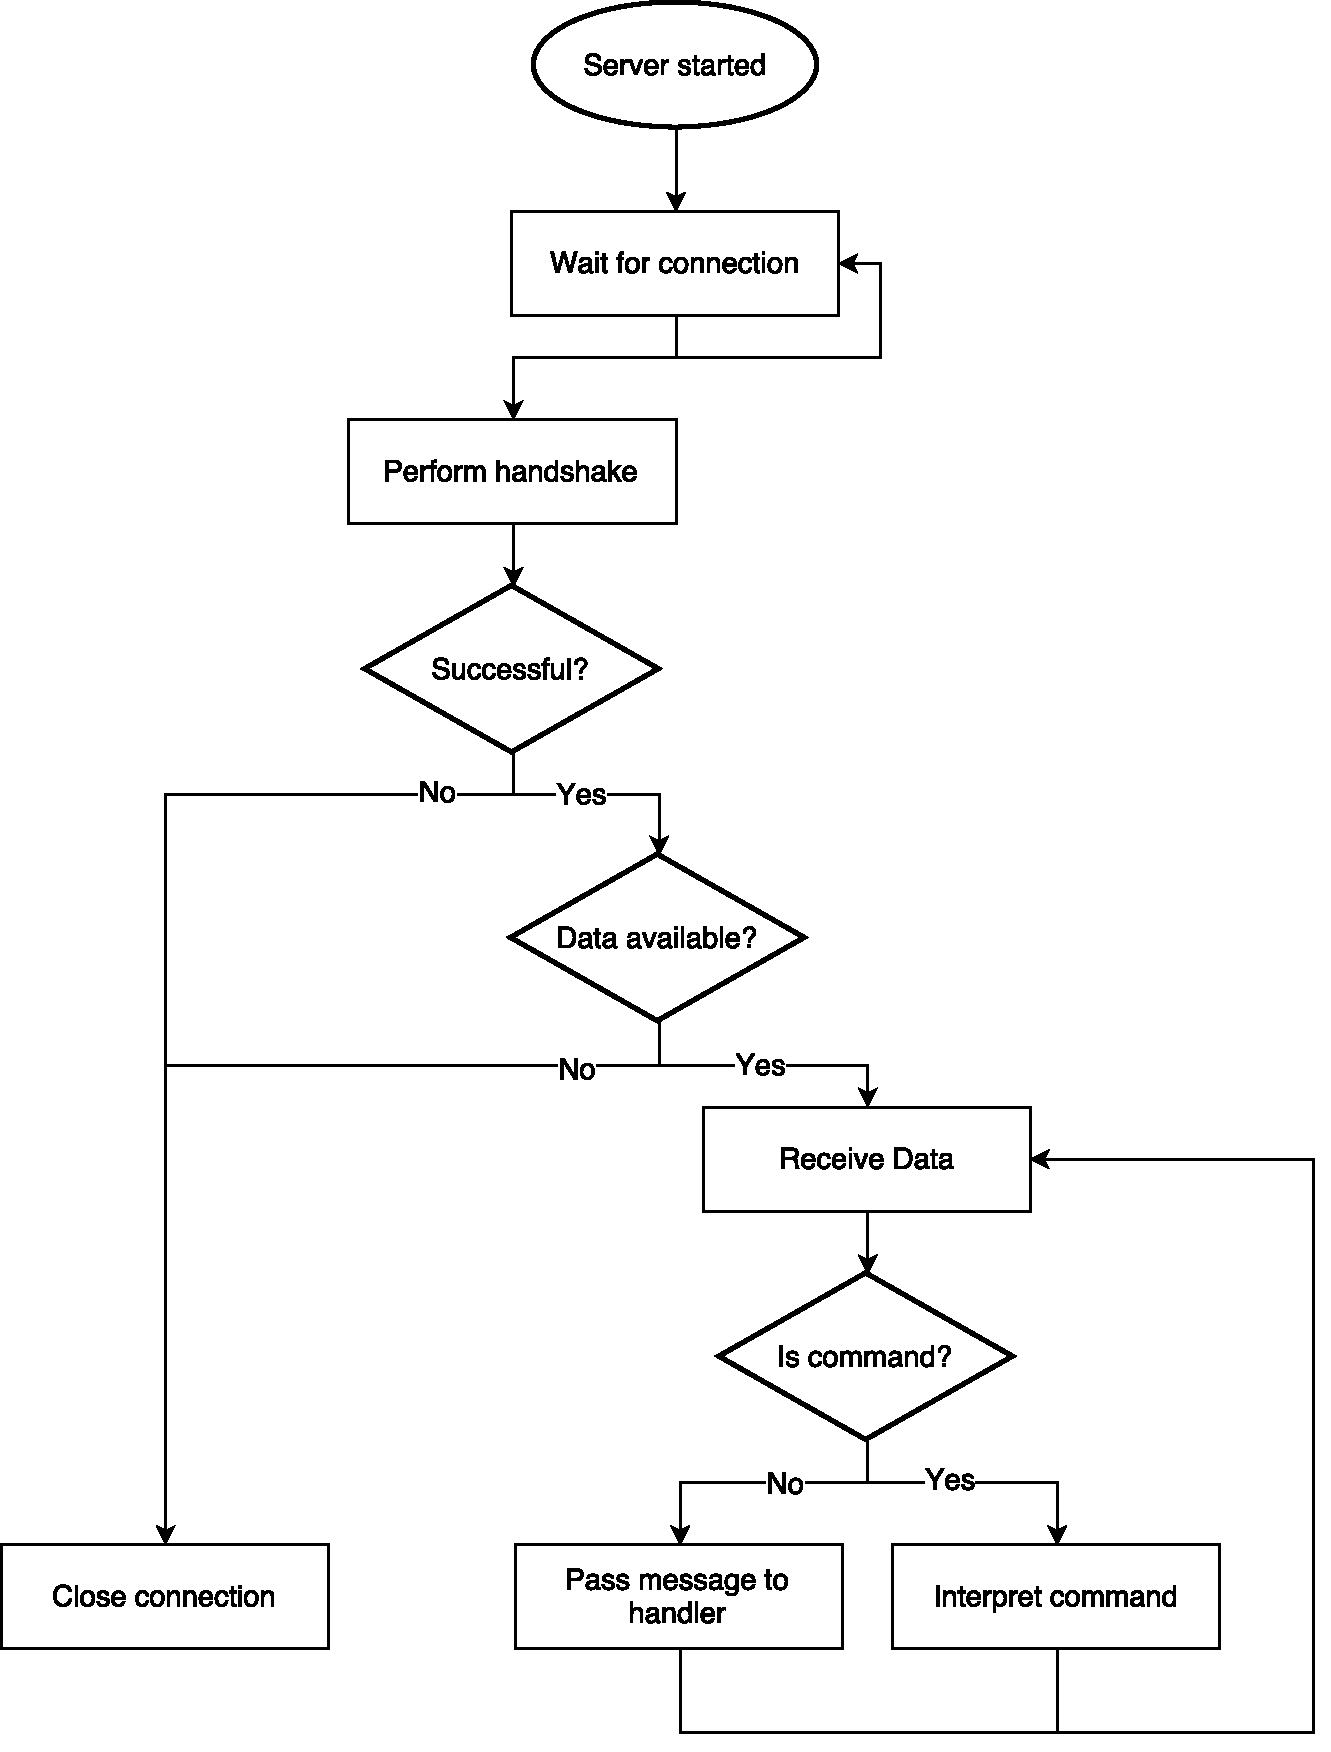
\includegraphics[width=13cm,keepaspectratio]{server-task}
	\caption{Flowchart of server program showing the procedure}
	\label{fig:server-program-flow}
\end{figure}

\chapter{Android}
\label{ch:Android}

\author{Nico Leidenfrost}
%
Android is a linux distribution and is currently developed by the software giant Google. Android is an operating system with primary focus on mobile devices with a built-in touchscreen. The most popular examples, in which Android is used, would be smartphones and tablets. Since Android is an open source project, developers all over the world can contribute to it and even build their own Android system. Android programs are called \textit{apps} which is the short version of application, these applications extend the basic functionality of an Android device.

\section{History of Android}
Android started as a startup Company under the name \textit{Android Inc.}, founded in October 2003, in the US city Palo Alto, California. At first its purpose was to serve as an operating system for digital cameras, that would be more advanced than the standard in 2003. One Year later in 2004 they changed their goals to focus on mobile phones instead of cameras because the market declined their approach. Google became aware of this company and acquired it in July 2005 along with its founding members. The first working prototype of an Android smartphone looked quite similar to a BlackBerry phone of the time, because it had the BlackBerry typical QWERTY keyboard. They made two versions of this prototype, both without a touchscreen. In 2007, Apple introduced the iPhone which already featured a touchscreen. Since then Google also focused on mobile devices that included a touchscreen, but also stated that a touchscreen could never fully replace physical buttons. The first officially sold Android smartphone that was the HTC Dream, launched in 2008. Google continued to maintain the Android project and launched many updates which introduced new features or just fixed existing bugs. The developers of Android did choose a quite funny naming scheme for their major releases, namely the names of desserts. Each version starting with ongoing letters from the alphabet starting with \textit{Cupcake} as the name for version 1.5. After that came version 1.6 called \textit{Donut} up to 7.0 as \textit{Nougat} and the latest version 8.0 as \textit{Oreo}. Google explained this naming scheme with the statement, ``Since these devices make our lives so sweet, each Android version is named after a dessert''.

\section{Design}
Material Design is Google's visual design language that was first introduced in 2014. The goal was to develop a single underlying system that allows for a unified experience across all kinds of devices. It tries to support visual elements with the characteristics of real materials, hence Material Design. These guidelines help the users to interact and quickly understand different kinds of User Interface (UI) elements by using familiar tactile attributes.

GRAMOC's Android app uses these design principles for the user interface as shown in figure \vref{fig:appscreenshots}

\begin{figure}[H]
    \centering
    \begin{tabular}{cc}
    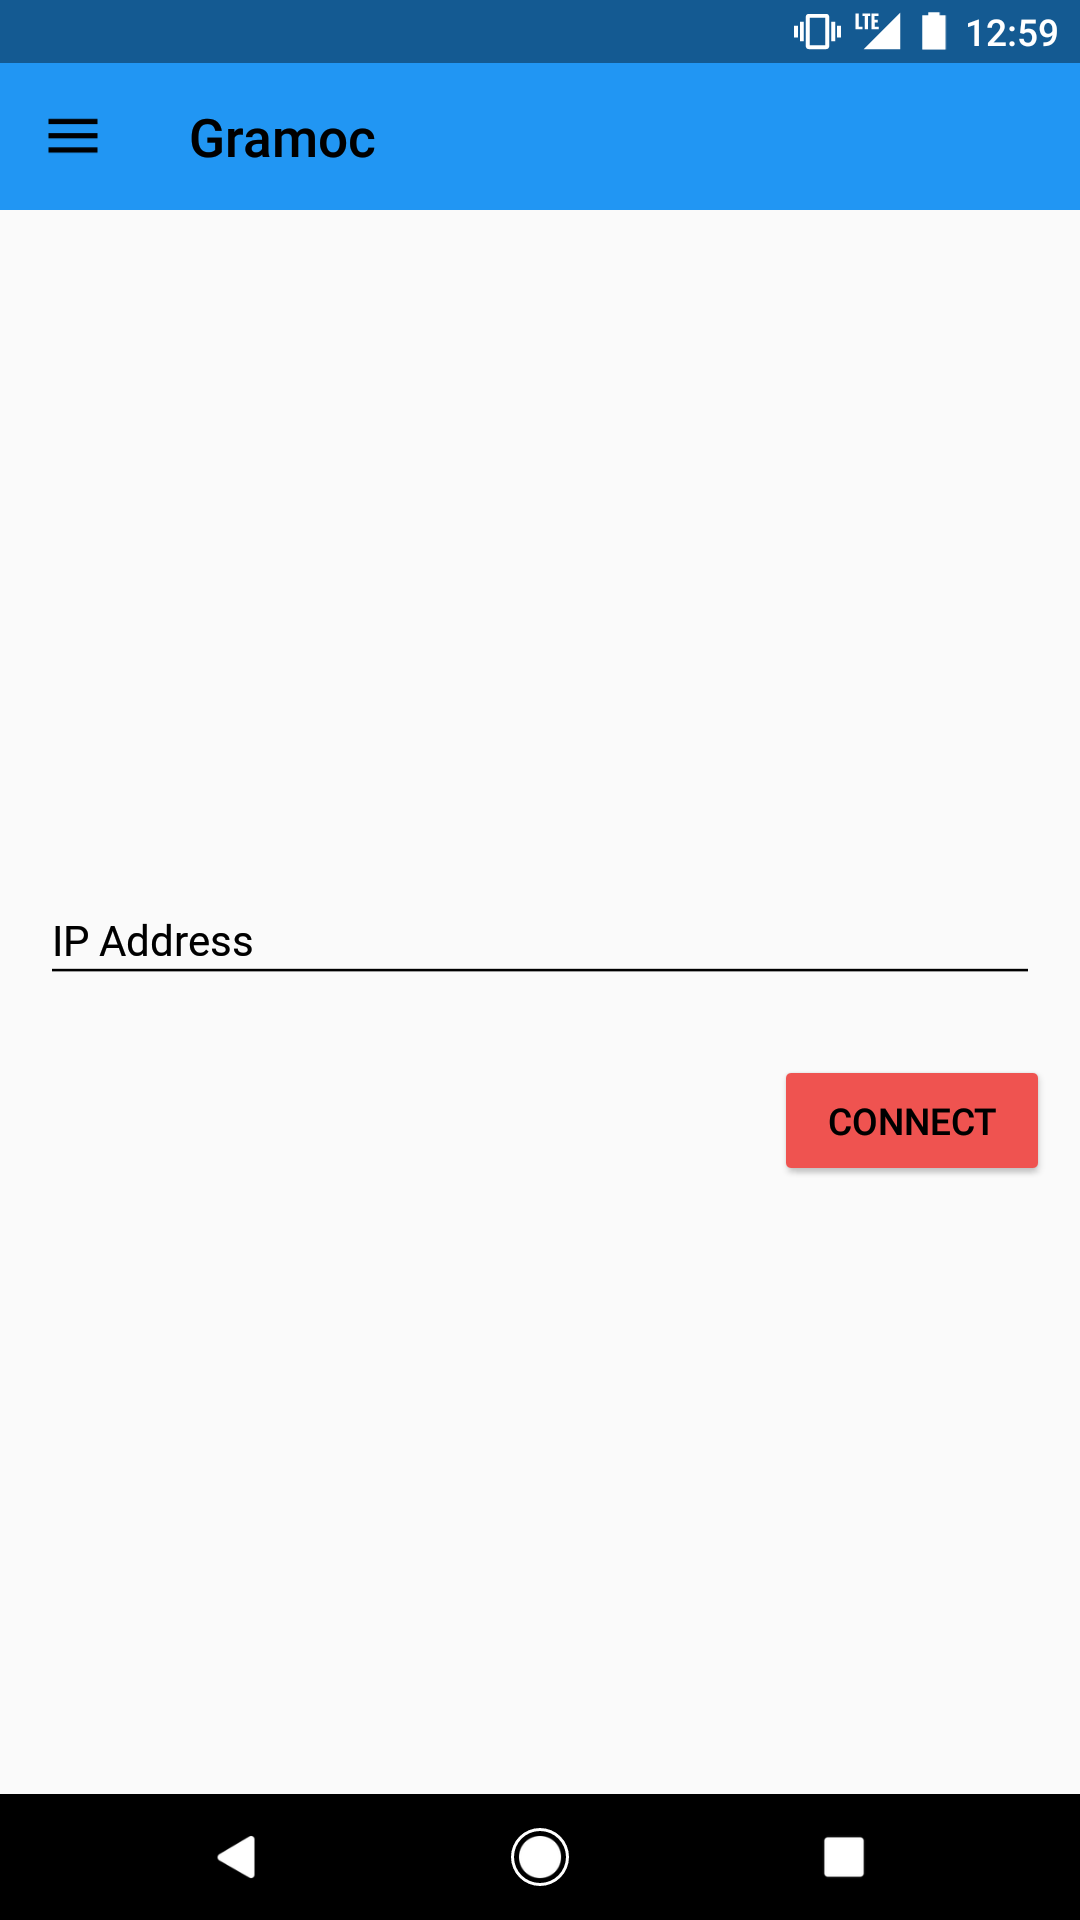
\includegraphics[height=7cm,keepaspectratio]{app_connect}
    &
    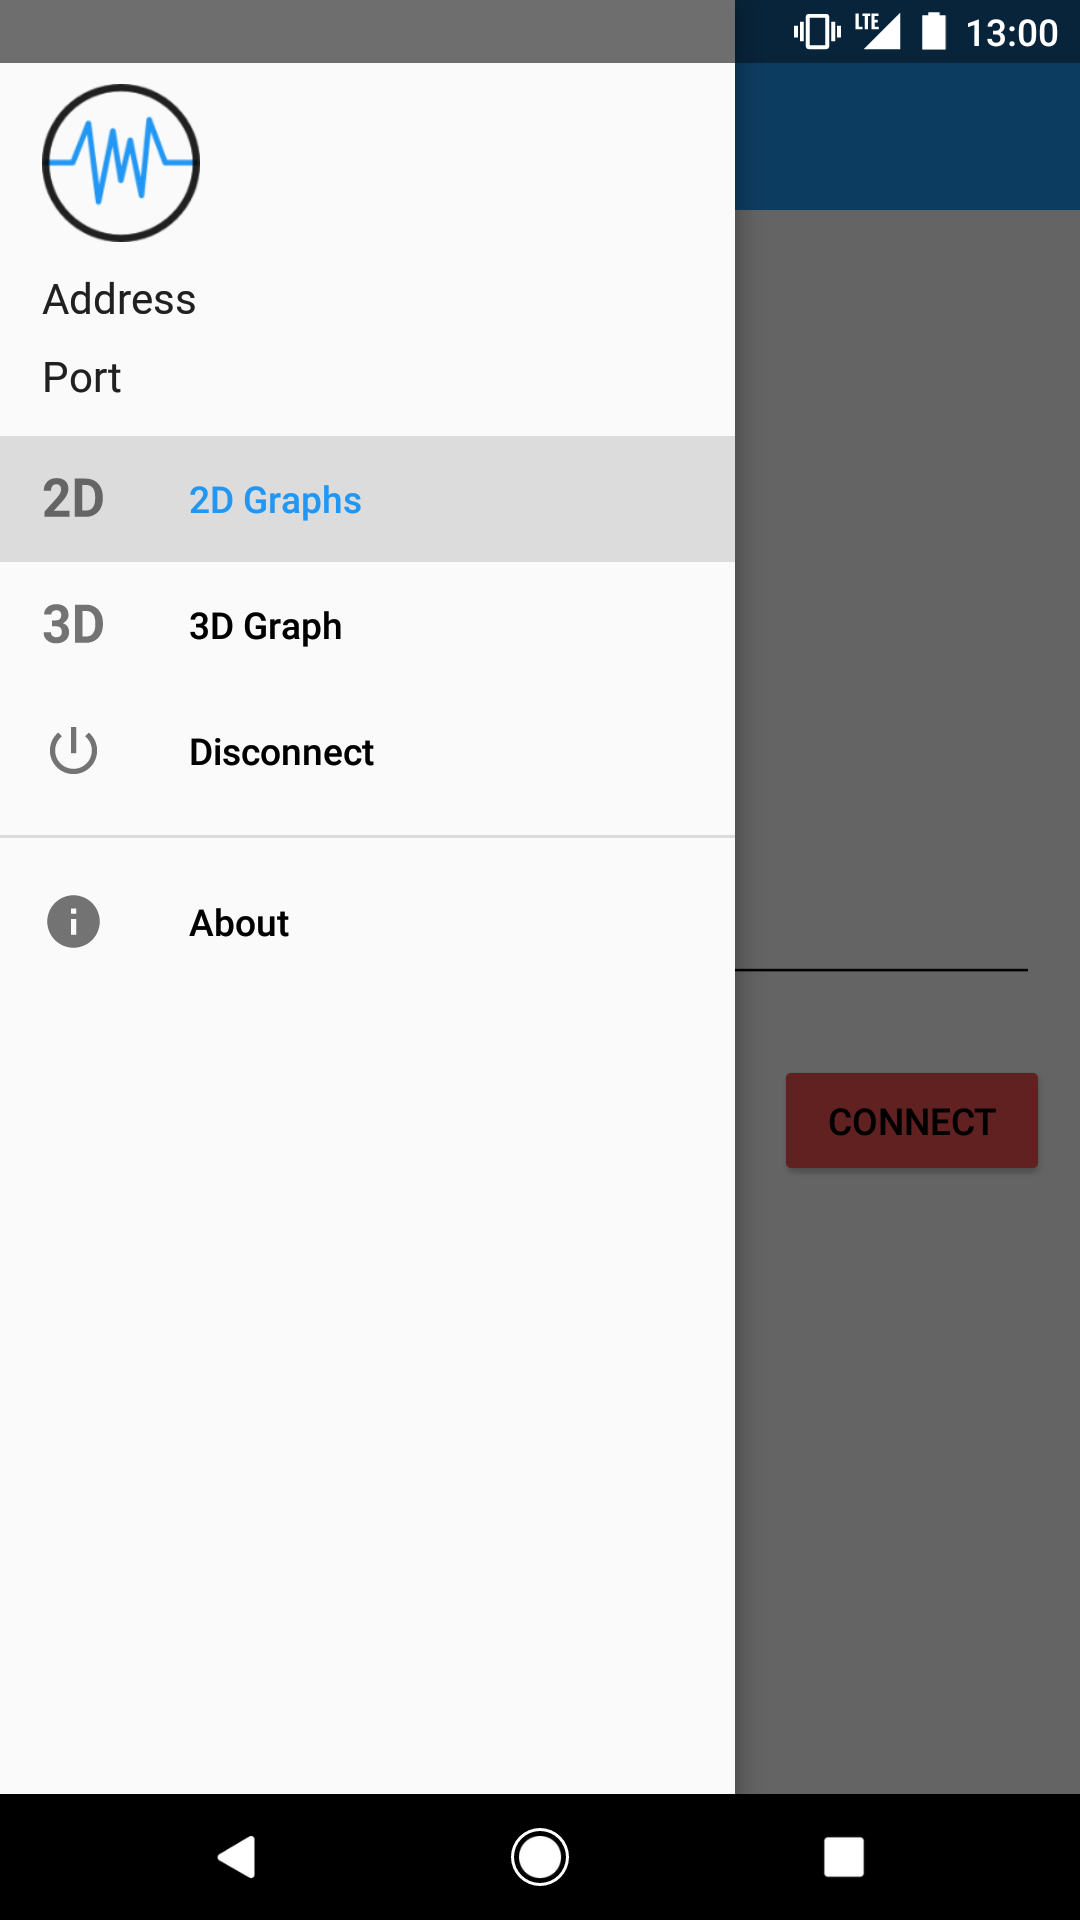
\includegraphics[height=7cm,keepaspectratio]{app_navdrawer}
    \\
    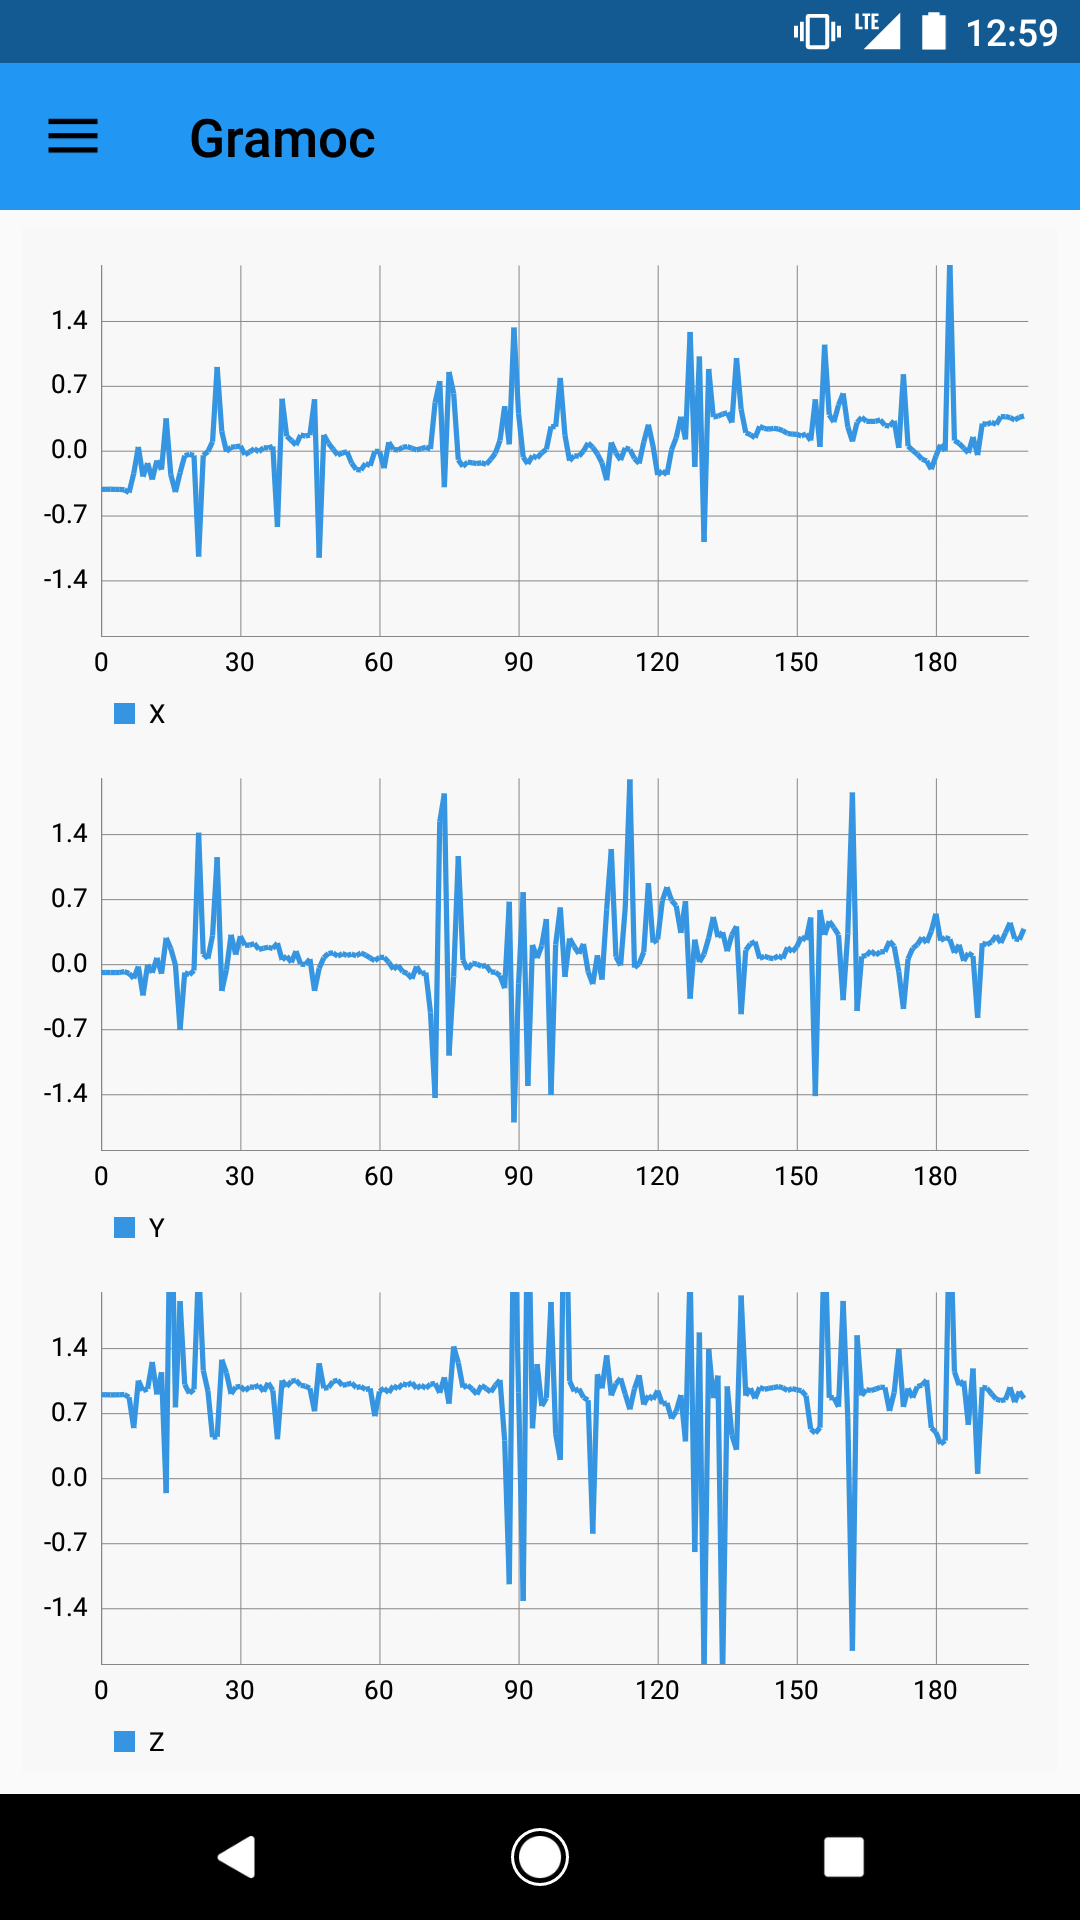
\includegraphics[height=7cm,keepaspectratio]{app_sensor}
    &
    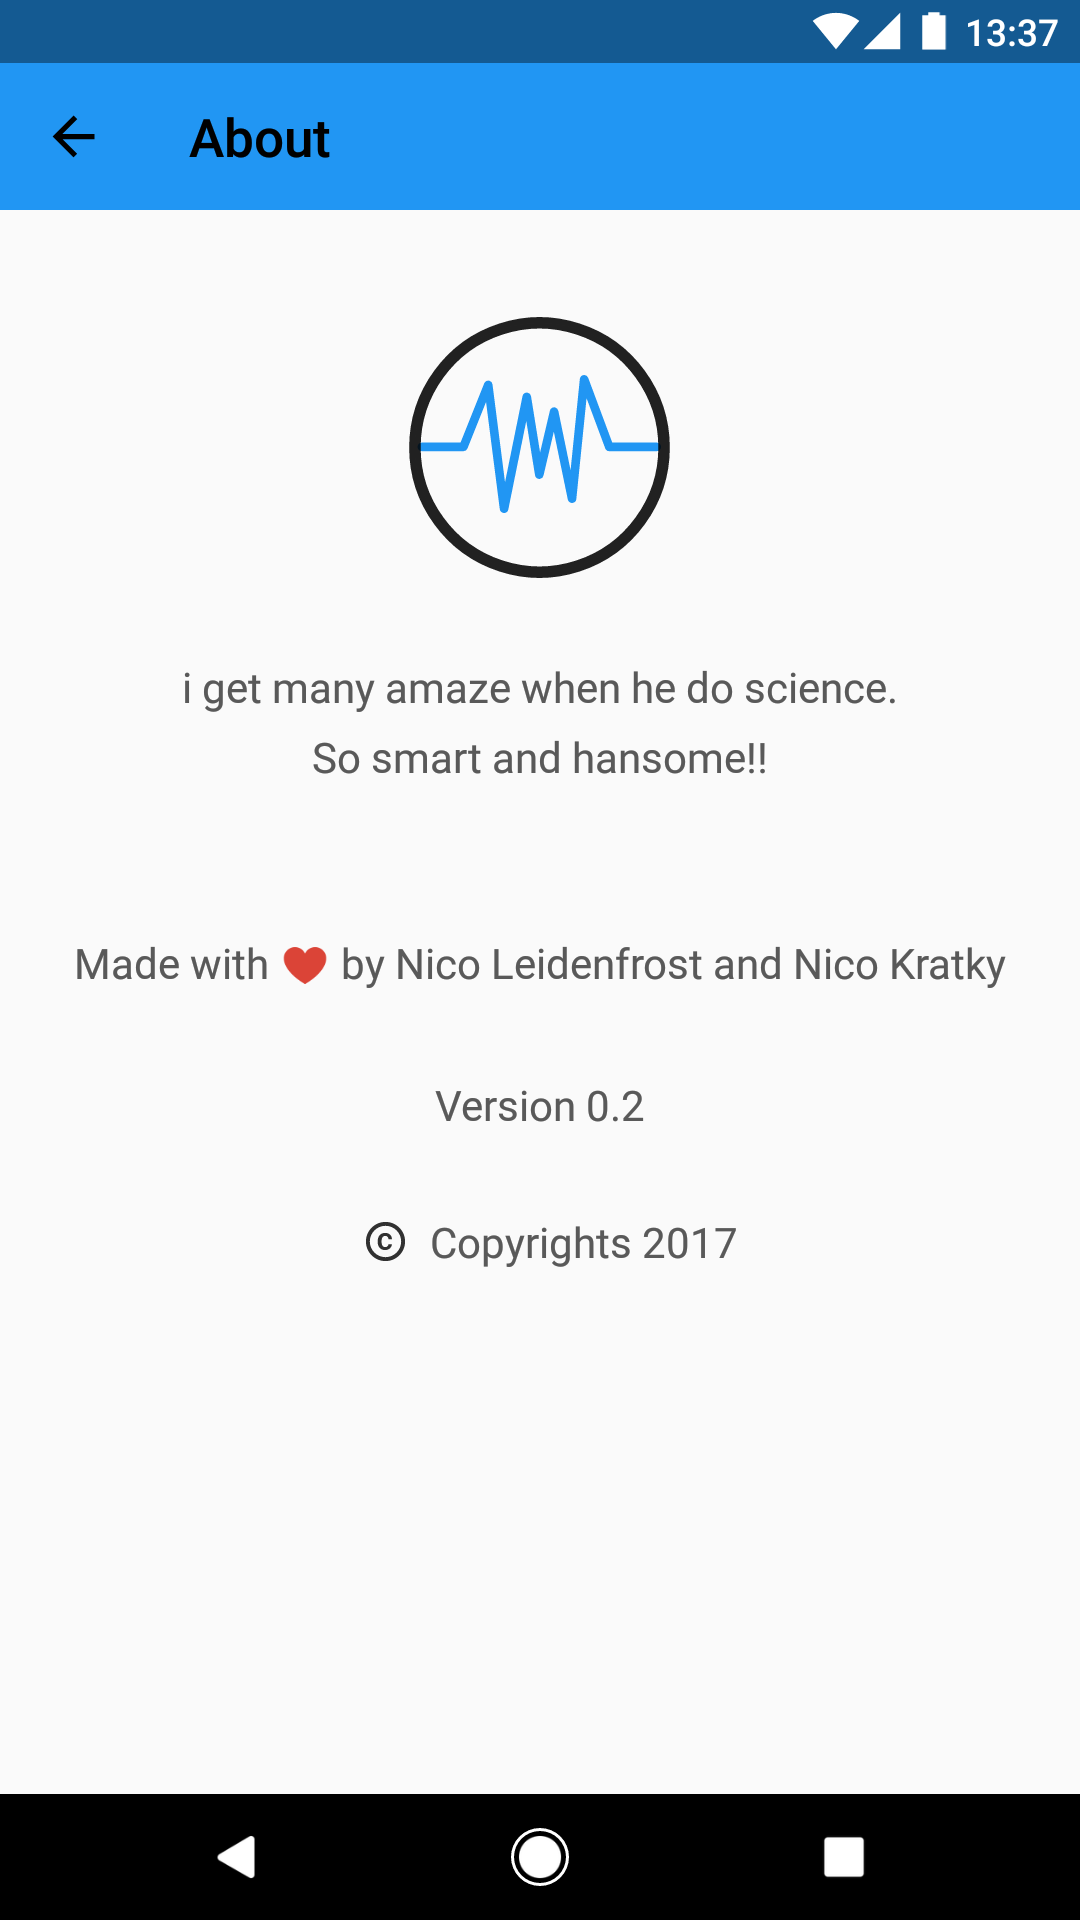
\includegraphics[height=7cm,keepaspectratio]{app_about}
    \end{tabular}
    \caption{Screenshots of App}
    \label{fig:appscreenshots}
\end{figure}

\section{Overview of Android Application Development}
Applications are often abbreviated as \textit{apps}. To write Android apps one must use the Android software development kit (SDK). The variety of programming languages that can be used is not very broad, so a developer must choose one of a few options to build a native Android app.

\subsection{Java}
Java is the most commonly used programming language to develop Android applications. The majority of apps and libraries are written in Java. These apps are compiled to bytecode which then will be translated to native instruction by the Android Runtime (ART). ART is an application runtime environment that replaced its predecessor Dalvik, a process virtual machine developed to run Android applications. Java was chosen to be the programming language to build the Android application in this project because of the broad variety of third-party libraries and support available.

\subsection{C/C++}
With C or C++ code and the Android native development kit (NDK), a native library for Android, applications can get much better results in terms of performance. The reason behind this is that the C/C++ code does not need a virtual machine to be executed (i.e. the code runs natively), therefore the performance of an application that uses C or C++ code can be much higher than the performance of an app written only in Java. Important is to mention that an Android application should not be written entirely in C/C++ because all the UI still needs to be handled by the Android framework and that is only available in Java. Since the Java native interface (JNI) handles the interoperability of the two languages, which adds a lot of complexity to the application, it would be best to only write functions that require a high CPU performance in C or C++ code.

\subsection{Go}
``The Go programming language is an open source project developed by a team at Google and many contributors from the open source community'' \autocite{GoProject}. This programming language is supported although there are limitations to the application programming interfaces (API), therefore it was not considered a reasonable option for GRAMOC.

\subsection{Kotlin}
Kotlin is a modern and powerful language, which is officially supported since May 2017 and solved various issues addressed with Java (e.g. Null references). Kotlin is interoperable with Java which means an Android application can contain both Kotlin and Java code. Kotlin was considered to be used in this project, but the fact that the official support was only recently introduced leads to less available third-party libraries as in Java. This led to the decision that Java was the programming language of choice.

\subsection{Runtime}
A runtime is needed to convert high level code written in languages like Java, into CPU readable byte code. Compiled Java code can not run on any machine because the code is compiled to Java byte code, which a CPU can not interpret. To run this Java byte code, the Java virtual machine (JVM) is needed, because it translates the Java byte code into CPU readable byte code. In Android however the Java code is compiled to Java byte code, then compiled again to Dalvik byte code and then given to the runtime. Android implemented a runtime called \textit{Dalvik}, which was later replaced by the \textit{Android Runtime Environment} \autocite{artanddalvik}.

\subsubsection{Dalvik}
The Dalvik Virtual Machine (DVM) was the first runtime used in Android. The DVM was chosen instead of the JVM to be used in the early days of Android because it could perform better when running multiple apps at once. Both virtual machines are quite similar to each other, except the matter that the JVM is stack-based and the DVM is register based, which means the DVM needs less instructions, but these must be more complex. At first Android devices only had a small amount of memory available, therefore the just-in-time (JIT) compilation of the DVM was a perfect concept because it resulted in a small memory footprint. This was achieved by only translating and caching the chunks of byte code that were needed to execute the next few steps of an application. So instead of compiling the whole code of an application, only the parts needed were compiled.

\subsubsection{Android Runtime Environment}
The problem of having to few memory available was solved by the fact that the hardware improved over the years. The primary focus of application developers changed from most efficient way to use memory to improve performance and simultaneously decrease battery usage. With that in mind the Android Runtime Environment (ART), which now uses Ahead-of-Time (AOT) compilation, was created. First introduced in Android 4.4 and later replaced Dalvik completely in version 5.0, ART increased the performance of Android application by compiling the whole code at once at the time of the installation of the app. This method improved startup time, battery consumption and overall performance, because now the code does not need to be compiled during runtime.

\section{Components}
In order to build this Android application following Android components were used:

\begin{itemize}
    \item Intent
    \item Toolbar
    \item Activity
    \item Service
    \item NavigationDrawer
    \item Threads
\end{itemize}

\subsection{Intent}
``An intent is an abstract description of an operation to be performed'' \autocite{AndroidIntent}. It handles the execution of a specific action that it takes along with data to operate on. It is most used when launching a new activity.

\subsection{Toolbar}
This component is a widget from the Android \emph{appcompat support library} and is persistent throughout the whole application. Most of the time it is referred to as app bar or action bar. Since this element is persistent, it will be used to perform important actions, like searching or navigating, but also to create space for identification of an application.

\subsection{Activity}
``An activity is a single, focused thing that the user can do.'' \autocite{AndroidActivity} Each application starts with launching an activity, therefore an activity handles the creation of a new window and loads all the User Interface (UI) elements. Activities are usually shown as a full-screen window, but also as a floating window or even be embedded inside of another activity by implementing an \textit{ActivityGroup}. Inside the Android-system, activities are handled as a stack, this means every time a new activity is launched, the Android system puts that activity on the top of the stack and this activity becomes the running activity. The other activities in the stack are placed below the active activity and therefore remain inactive. An activity's lifecycle can be understood as depicted in figure \vref{fig:activitylifecycle}.

\begin{figure}[H]
    \centering
    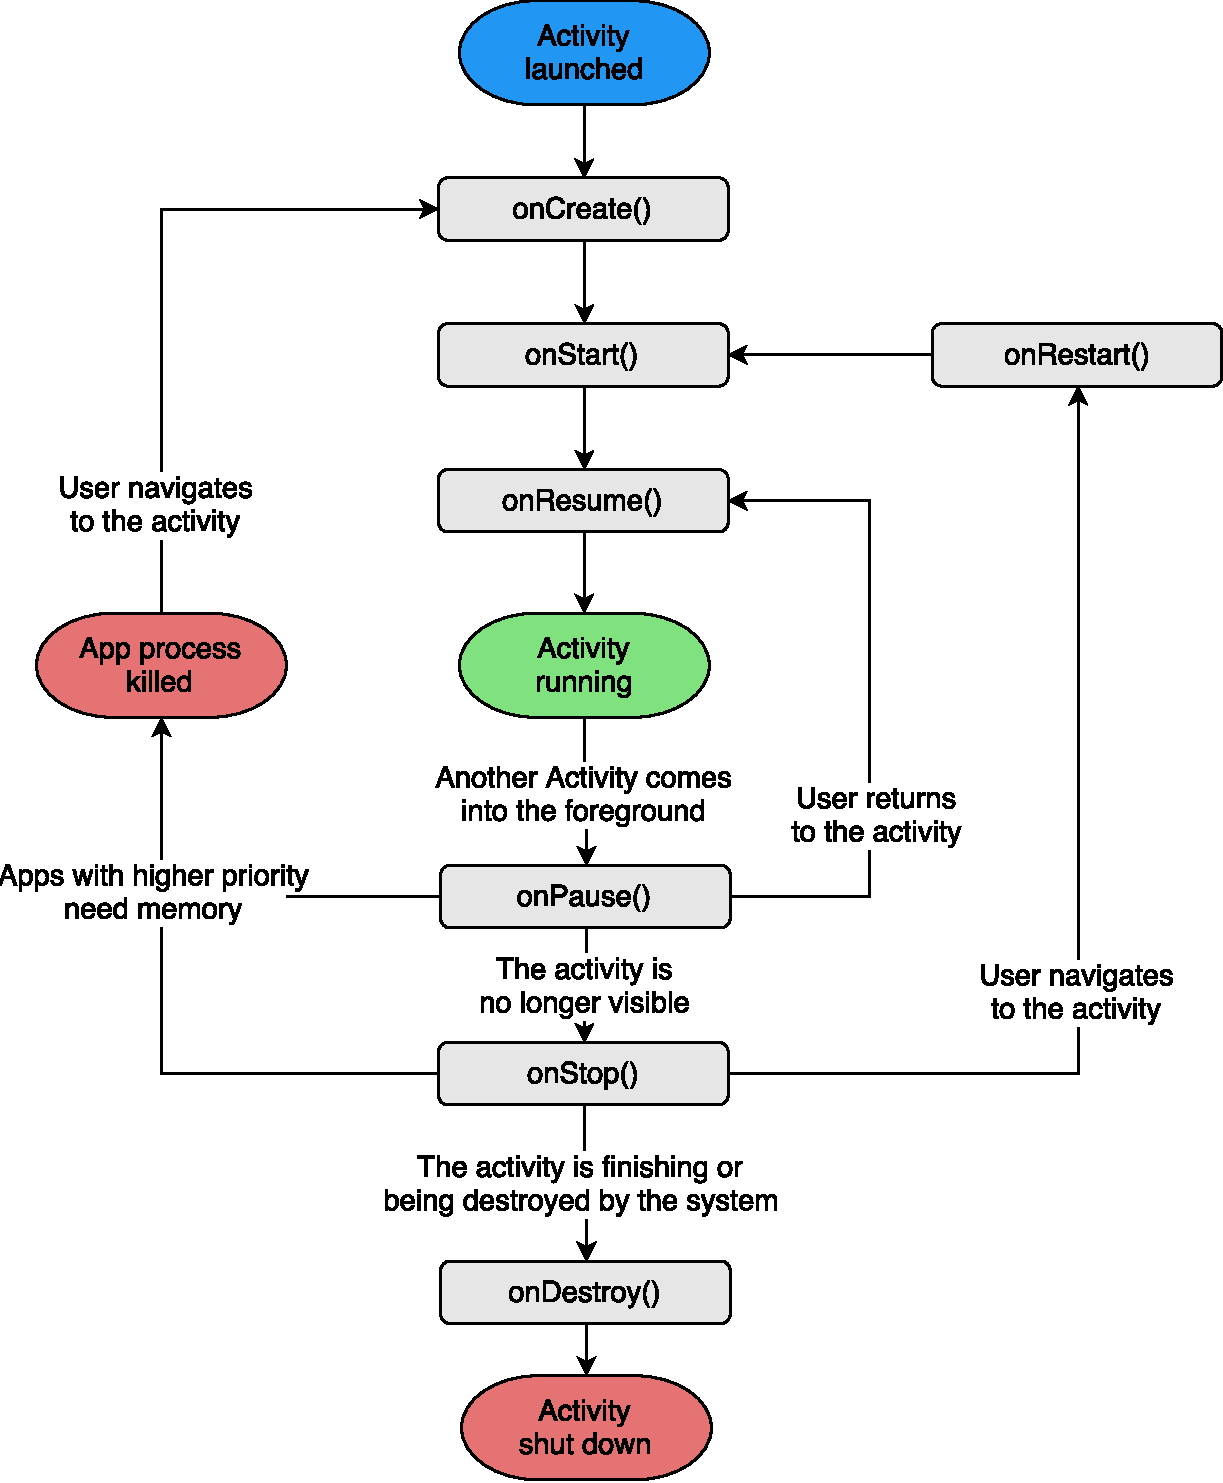
\includegraphics[width=10cm,keepaspectratio]{android-activity-lifecycle}
    \caption{Flowchart showing the lifecycle of an Android-activity}
    \label{fig:activitylifecycle}
\end{figure}

\subsection{Service}
A service in Android can be compared to a daemon. It is a process that runs in the background and therefore there is no need for a visual interface. Once started, a service can persist in the background and is therefore not interrupted by switching applications. To use a service within another component, it must bind the service to enable interprocess communication (IPC). The most common application of a service is, handling network connections. The lifecycle is defined as depicted in figure \vref{fig:servicelifecycle}.

\begin{figure}[H]
    \centering
    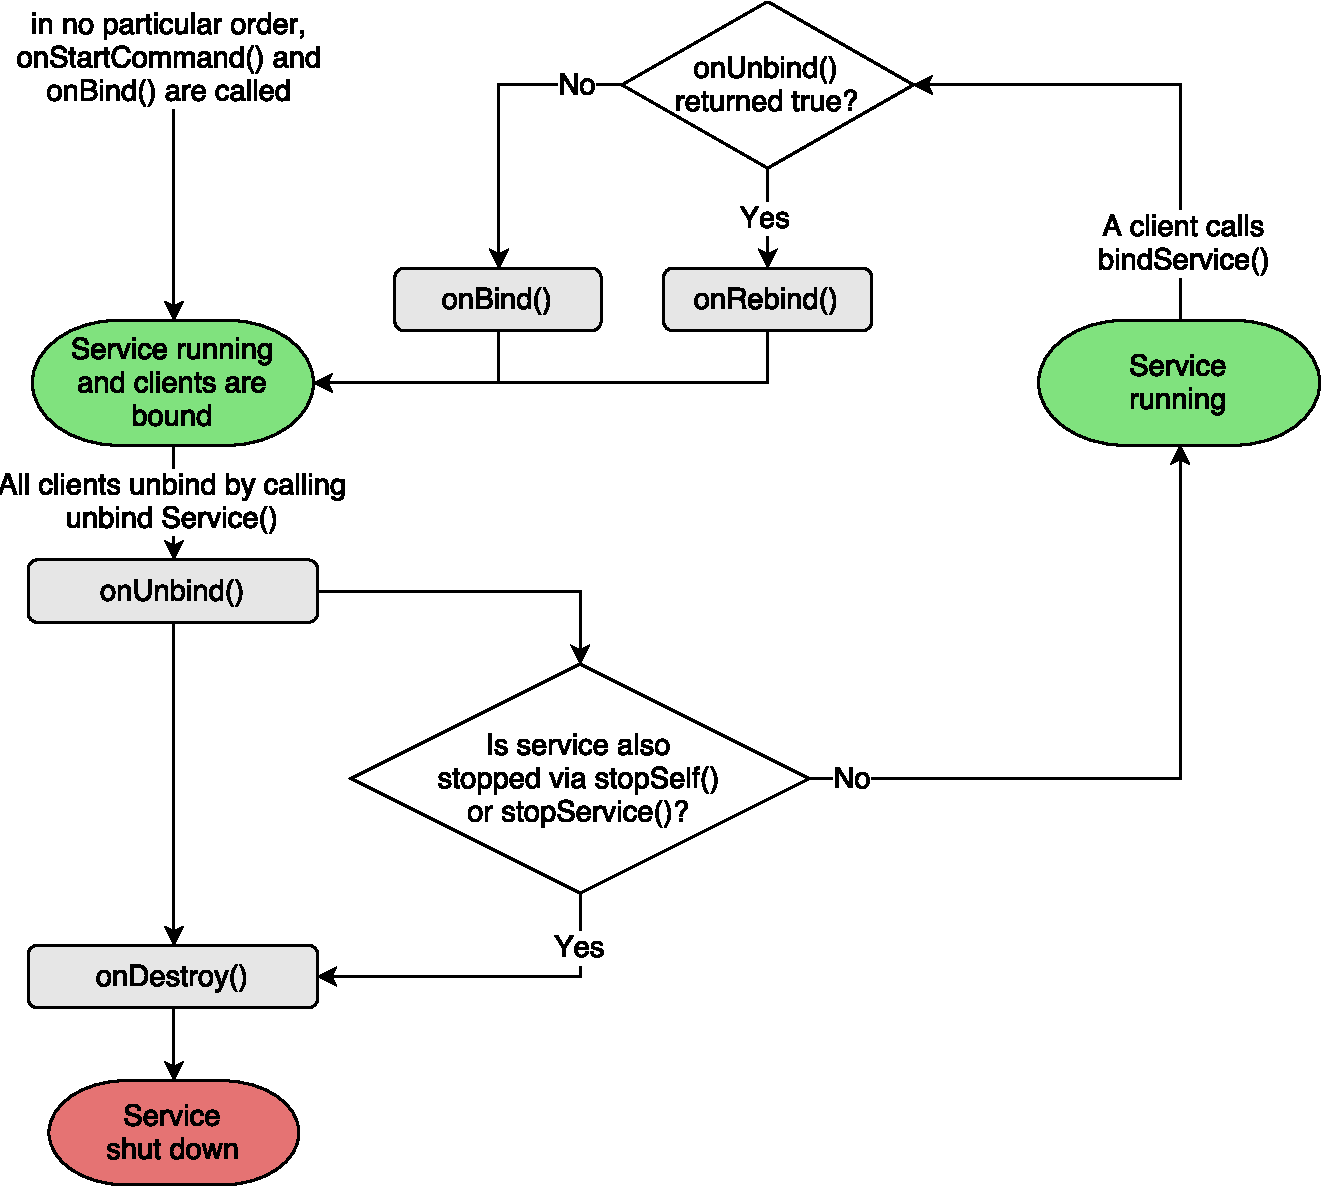
\includegraphics[width=10cm,keepaspectratio]{android-service-lifecycle}
    \caption{Flowchart showing the lifecycle of an Android-service}
    \label{fig:servicelifecycle}
\end{figure}

\subsection{NavigationDrawer}
To navigate between the activities and views a navigation drawer was implemented. A navigation drawer is a panel which is pulled from the left border of the screen to approximately 3 quarters of the screen width. It contains a header where general information is displayed and a body which contains various navigation items. The navigation drawer is included in the material design pattern, which is often used in Android application development, so most Android apps provide a navigation drawer.

\subsection{Threads}
When an Android application component is launched and it is the first component of an application, Android will start a new Linux process. If this application is already running inside a process and a new component is launched or an action is preformed, Android will execute this task in the main-thread of the application. Unless it is explicitly stated to execute the operation in a new thread within this process. When working with threads in Android two essential rules must be followed \autocite{AndroidThreads} :

\begin{enumerate}
    \item Do not block the UI thread
    \item Do not access the Android UI toolkit from outside the UI thread
\end{enumerate}

\noindent The reasons behind this two rules are quite simple. The point why the thread that contains the user interface should never be blocked is simply because then, no events could be dispatched, including events that update the UI itself. This would mean that the application could not give any information to the user unless the operation which is blocking the thread has finished. This is really bad, because the user could think that the application stopped working. Accessing the UI toolkit from a thread other than the UI thread is also a bad idea, since the UI toolkit is not thread-safe. This means if multiple threads would access UI elements, race conditions could happen and therefore cause errors within the application. To avoid such errors Android implemented different ways how to execute tasks asynchronously in Android:

    \subsubsection{Extended Threads}
    The first way is to implement a subclass of the Java \emph{Thread} class. If this solution is chosen a developer must override the \emph{run} method of the superclass. If the way of how a thread handles certain situations needs to be changed or new functionalities needs to be added, a developer should choose this method, otherwise the Runnable interface should be implemented.

    \subsubsection{Runnable interface}
    Another method to accomplish asynchronous behaviour would be to implement the \emph{Runnable} interface when creating a class. To execute the tasks, an instance of this class needs to be given to the thread which should execute the tasks. This way is preferred to use when running tasks which does not need modified thread behaviour. When tasks from a runnable class are executed there is no need to launch a new thread for each task, instead they can be executed on various threads.

    \subsubsection{AsyncTasks}
    AsyncTasks are implemented to move work to the background and then update the UI accordingly. An AsyncTask is defined to execute blocking operations, therefore there will be only one active AsyncTask at the same time. In order to perform an AsyncTask a cycle of four tasks is executed, with following steps:

    \begin{enumerate}
        \item \textbf{onPreExecute}: executed on the UI thread before the task is executed.
        \item \textbf{doInBackground}: executed on the background thread, here the background tasks are executed.
        \item \textbf{onProgressUpdate}: executed on the UI thread every time when \emph{publishProgress} is called in the background thread.
        \item \textbf{onPostExecute}: executed on the UI thread when the background tasks are finished.
    \end{enumerate}

\subsection{Libraries}
The Android client was implemented using a small number of libraries:
\begin{itemize}
    \item \textbf{Android SDK}

    The standard libraries included in the Android platform itself \autocite{AndroidSDK}.

    \item \textbf{GramocAlgorithm-client}

    The Java implementation of the GSDEP client developed along with this project \autocite{GramocAlgorithm-client}.

    \item \textbf{MPAndroidChart}

    An easy to use but also powerful open source 2 dimensional chart library for Android \autocite{MPAndroidChart}.

    \item \textbf{android-about-page}

    This library allows to simply create an about page for your Android application \autocite{android-about-page}.
\end{itemize}

\section{Implementation}
The entry point of this Android application is called the \emph{MainActivity}. When this Activity starts a background service is additionally started, which is basically a wrapper for the GSDEP client, therefore it handles all the networking related tasks within the app. The service will be bound to the active activity, so every time another activity is launched the service will be unbound by the current activity and newly bound by the starting one. The \emph{MainActivity's} goal is to give the user an easy way to connect to the server. Once the application successfully connected to the server, a new activity responsible for plotting the received sensor data will be launched, whether the 2-dimensional or the 3- dimensional plotting activity is launched depends on the selection made in the \emph{NavigationDrawer}, by default the 2-dimensional plotting activity will be launched. When the 2-dimensional plotting activity is launched the networking service will be bound and three \emph{LineCharts} contained within the library \emph{MPAndroidChart} will be created and properly set up. After these tasks are finished and the activity is ready to receive data, the server will be notified. Now each data set received will be added to the data buffer of the respective chart. If the buffer of a chart is full, the values at the end will be truncated until there is enough space to add the new values. The 3-dimensional plotting activity however was not implemented at all, since the Android application was discontinued because of problems that appeared during the development of the 2-dimensional activity (see chapter \vref{ch:Problems}).


\part{Lessons Learned}
\chapter{Problems}
\label{ch:Problems}

After extensive testing it was decided that this approach will not lead to successful project outcome. This decision was made while taking several factors into consideration.

\section{Android}
Android is a great platform to create simple and even complex application systems that does not rely on heavy performance. Since the key element in this project is the ability to display the sensor data in real time, the Android development was discontinued due to the performance issues that come with it.

\section{Software limitations}
Android is designed to render the UI with 60 frames per second (fps), which results in redrawing frames every 16 milliseconds at best. The task of drawing frames will be executed by the main thread along with many other operations like system events, input events, application callbacks and so on. The system tries to update the screen every 16 milliseconds, if however other operations than the redrawing of the screen are pulled from the work queue when trying to update the screen these frames will simply be dropped and users will experience lacks of smoothness while using the application. To be sure about how much milliseconds the rendering of one packet takes the time was stopped. The results showed that it took up to about 50 milliseconds to to render one update. These measurements were the prime factor that led to the decision to discontinue the work on Android.

\section{Plotting Libraries}
There are a lot of freely available plotting and charting libraries to use in Android development. Unfortunately most of them do not meet the requirements to be used in this project. There are many good libraries to plot 2 dimensional charts like pie charts or bar charts, but there is a lack of libraries that can display scientific plots (e.g. surface plots). The libraries that would meet all the requirements however are not originally designed to be used in Android development and therefore work only in specific version of Android or do not work at all because they rely on components that are not available in Android.

\chapter{Conclusion}
After researching alternatives that still fit the purpose of GRAMOC a meeting with the client was arranged to discuss these alternatives. This meeting resulted in new goals and expected results. This new project specification now includes a web application instead of the mobile Android application.

\section{Advantages}
The switch to developing a web application still offers a few advantages that were not existing while focusing on a Android application. This includes the flexibility as a web application can run on basically any devices the end user wishes. As of today many devices support network connections and can run a web browser. Another advantage is that JavaScript offers a tremendous amount of third party libraries, especially plotting libraries. There a also a few libraries that support scientific plotting, even VTK the visualization toolkit that is used by ParaView is available as a JS version \cite{VTK}.

\section{Disadvantages}
The change of specifications also brings some disadvantages with it. For example the whole networking stack has to be rewritten because raw TCP streams are not supported in web environments. They were replaced be the WebSocket technology \cite{rfc6455}. Also a new third-party plotting library has to be chosen and read up on.


\part{Implementation Phase 2}
\chapter{Software Architecture}
\label{ch:Software_Architecture}

\author{Nico Kratky}
%

After studying lots of literature about real-time systems, a new fundamental software architecture was developed. The main principle of this is to seperate different tasks into seperate processes. This makes use of the fact that the processed data is sent to the client over the internet anyways. Therefore the process that handles data storage also acts as a client. This leads to increased protability, and more important, increased performance. This sofware stack is depicted in figure \vref{fig:gramoc-stack} and its components are further introduced and discussed in the following chapters.

\begin{figure}[!htb]
    \centering
    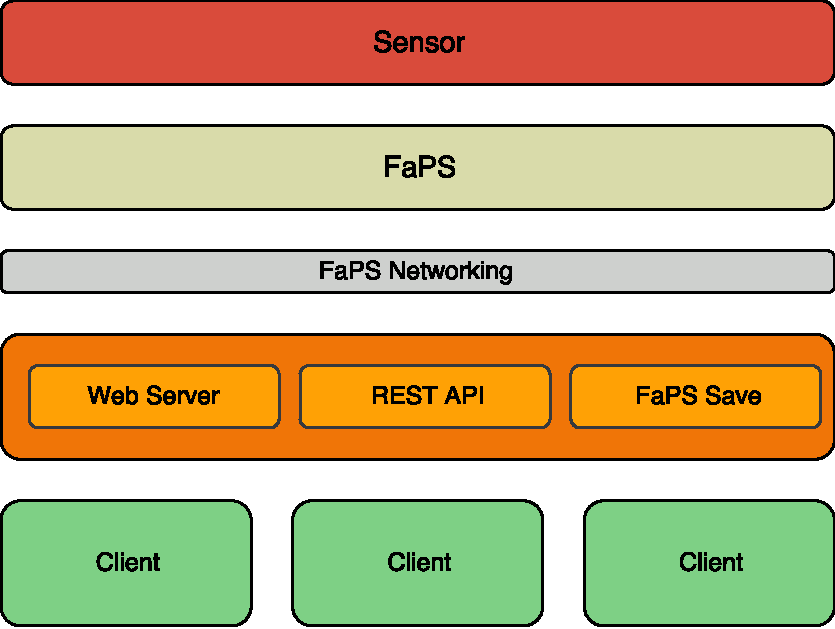
\includegraphics[width=10cm,keepaspectratio]{gramoc-stack}
    \caption{GRAMOC Software Architecture Diagram}
    \label{fig:gramoc-stack}
\end{figure}


\chapter{FaPS Networking}
\label{ch:faps-networking}

\author{Nico Kratky}
%

FaPS Networking is a custom UDP-based library that is mainly used for communication between FaPS (see \ref{ch:faps}) and different kinds of client, eg. FaPS-save (see \ref{ch:faps-save}) and the NodeJS server (see
\ref{sec:webserver}).

\section{TCP vs UDP in real time environments}

% comparison between TCP Header and UDP Header -> more Overhead -> more Information
% TCP -> feedback mechanism, not relevant in real time environments, when dropped packets are resent they are outdated and not relevant -> don't care when dropped
% TCP is perfect for transferring big files bc when one byte is missing whole file is corrupt
% reliability comes at cost -> much larger overhead!
%
% include images of headers!!!!

\cite{TCPUDPRTlifesize}

\todo{cite whole paragraph like this?}

\section {Handling Connections}

As UDP is a connectionless protocols, neither does it know if the other end of the communacation is ready to receive data nor if it is even existing. Therefor a way of handling connections using UDP had to implemented.

The core of this implementation is a map. A map is a associative container that is available through C++'s STL (Standard Template Library). This maps contains all clients as keys, and the associated timestamps of the last
received keepalive message as values.

After starting the server, two threads are started. The first one handles all incoming messages. If a received message is a keepalive message the timestamp of the client that sent this message is update
to the current time. The second thread monitors these timestamps. If the difference between the current timestamp and the stored timestamp of a client exceeds 1.5 seconds, the client is declared disconnected and removed
from the list.

Also when a client is instantiaed a thread is started to handle the keepalive messages. The only task of this thread is to send a keepalive message to the server and then wait one second. All of this is done in a loop that
only finishes when the clients deconstructor is called, thus disconnects.

\section {Handshake}

The handshake procedure is a very important part of connecting. This makes sure that the server is notified whenever a client is waiting to connect.

When the server receives a connection request (see \ref{tab:faps-networking-control-messages}), it has to check if it can accept further clients. This limit is set as a static constant in the \textit{Server} class. The
default value is \textbf{8}. If this check is successful the server sends an acknowledgement message to the client. If the check fails, the client will receive a connection refused message. In this implementation the
clients connect call will block until it is connected. This is done by a loop that will be exited once the server sends an acknowledgement. In between the connection attempts one second is waited.

These two procedures can be both seen in the code listings (\ref{lst:faps-networking-handshake-server} and \ref{lst:faps-networking-handshake-client}) and the sequence diagram (\ref{fig:faps-networking-handshake}) below.

\begin{minipage}{\linewidth}
\begin{lstlisting}[caption={Server handshake method}, label=lst:faps-networking-handshake-server, captionpos=b, language=C++]
void Server::shake_hands(boost::asio::ip::udp::endpoint& remote) {
    if (endpoints_.size() < MAX_CLIENTS_) {
        send(control_messages["ACKNOWLEDGE"], remote);
        endpoints_[remote] = std::chrono::system_clock::now();
    }
    else {
        send(control_messages["CONNECTION_REFUSED"], remote);
    }
}
\end{lstlisting}
\end{minipage}

\begin{minipage}{\linewidth}
\begin{lstlisting}[caption={Client handshake method}, label=lst:faps-networking-handshake-client, captionpos=b, language=C++]
void Client::connect() {
    while (!connected) {
        send(control_messages["CONNECTION_REQUEST"]);

        std::string reply;
        receive(reply);

        if (reply.compare(control_messages["ACKNOWLEDGE"]) == 0) {
            connected = true;

            std::thread t_keepalive{&Client::keepalive, this};
            t_keepalive.detach();
        }
        else {
            std::this_thread::sleep_for(TIMEOUT_);
        }
    }
}
\end{lstlisting}
\end{minipage}

\begin{figure}[H]
    \centering
    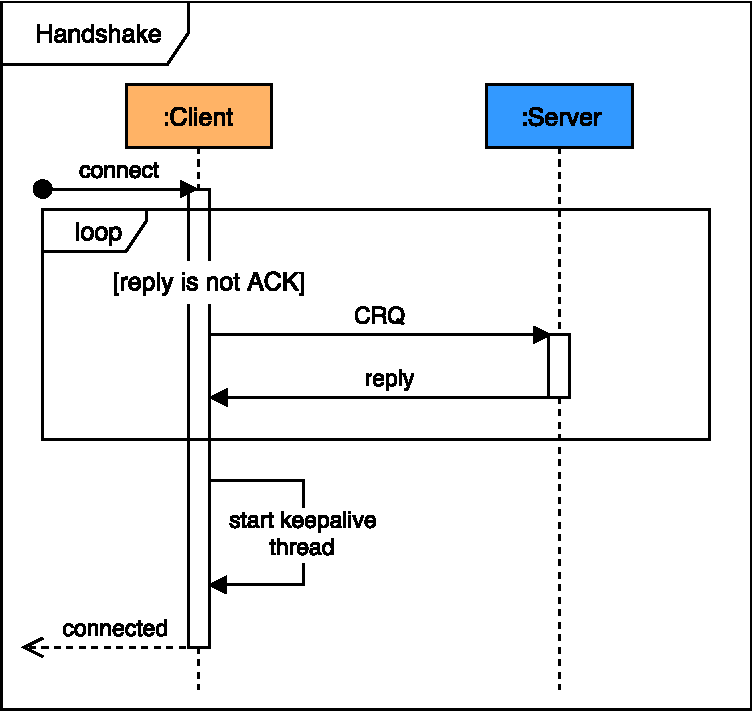
\includegraphics[width=8cm,keepaspectratio]{faps-networking-handshake}
    \caption{Handshake performed when a client tries to connect to server}
    \label{fig:faps-networking-handshake}
\end{figure}

\section{Control Message}

This table explains all control messages that can be exchanged.

\begin{table}[H]
    \centering
    \begin{tabular}{| l | l | p{5cm} |}
    \hline
    \textbf{Message} & \textbf{Sent to} & \textbf{Meaning} \\ \hline
    CRQ & server & Tells the server that a new client is waiting for the connection procedure \\ \hline
    ACK & client & Tells the client that the connection is acknowledged \\ \hline
    CRF & client & Tells the client that the server can not accept the connection \\ \hline
    KAV & server & Tells the server that the client is still alive and wants to stay connected \\
    \hline
    \end{tabular}
    \caption{Commands sent by one of the connection partners and what they do}
    \label{tab:faps-networking-control-messages}
\end{table}


\chapter{Filtering and Preprocessing System}
\label{ch:faps}

\author{Nico Kratky}
%
The main task of GRAMOCs Filtering and Preprocessing System, also known as simply FaPS, is to read digital sensor output, preprocess it and forward it to another process that handles the distribution.

\section{Command Line Parameter Parsing}

As FaPS is a command line program arguments that are passed to it have to be parsed. This is done by Boosts program\_options \cite{BoostProgramOptions}. This module allows easy parsing and exception handling.

Following arguments can be passed to FaPS:

\begin{table}[H]
    \centering
    \begin{tabular}{| l | l | p{5cm} |}
    \hline
    \textbf{Flag} & \textbf{Argument} & \textbf{Meaning} \\ \hline
    -h, --help & & Outputs the usage information \\ \hline
    -i, --ip & \textit{ip\_adress} & Sets the IP address to which FaPS will connect to read sensor data \\ \hline
    -p, --port & \textit{port} & Sets the Port to which FaPS will connect to read sensor data \\ \hline
    -f, --file & \textit{filename} & Sets the filename to which the data will be saved \\
    \hline
    \end{tabular}
    \caption{Flags that can be set, which arguments they take and what they do or change}
    \label{tab:faps_arguments}
\end{table}

\section{Networking}

All networking related programming was done by utilizing Boosts Asio module. Asio is a cross-platform C++ library for network programming. The main feature is its asynchronous I/O model \cite{BoostAsio}.

\todo{Explain Boost::Asio more precise}

\section{Data Storage}

To be able to offer a possibility for further data inspection all received data is saved to a HDF5 file. HDF stands for Hierarchical Data Format. It is a file format for storing large amounts of scientific data. A HDF5 file is organized hierarchically as the name suggests. This is achieved by following a tree structure and dividing the data into groups and datasets. The format of a HDF file can be compared to a file system with the exception that HDF groups are linked as a directed graph. This means that a HDF file allows circular references.

\section{Data Serialization}

\todo{Rework whole section (JSON instead of protobuf)}

In order to send data so that the other end can interpret the message it has to be packed into a common format. To do this Googles protobuf libary is used \cite{Protobuf}. This is a language- and platform-independent data serialization library developed by Google. Data structure is defined in a \textit{.proto} file. With the help of special generated source code it is easy to interact with this specified data structure.

\begin{lstlisting}[caption={The \textit{.proto} file used by GRAMOC}, captionpos=b]
syntax = "proto3";

package gramoc;

message SensorPacket {
    repeated sint32 channel_1 = 1;
    repeated sint32 channel_2 = 2;
    repeated sint32 channel_3 = 3;
    repeated sint32 channel_4 = 4;
    repeated sint32 channel_5 = 5;
    repeated sint32 channel_6 = 6;
}
\end{lstlisting}

\section{Data Forwarding}

When the sensor data is packed to a binary format using protobufs it has to be passed to another process on the same host. This is a typical use case for inter-process communication. It was decided to use normal UNIX domain socket for this. In the case of GRAMOC FaPS has the server role and the processes that handle end-client connections are clients.

\todo{describe unix domain sockets}

\chapter{Saving Sensor Data}
\label{ch:faps-save}

\author{Nico Kratky}
%
In order to be able to look up recent sensor readouts, all data that is received from the sensor has to be saved in a persistent way. This chapter introduces the program that was implemented to solve this task.

\section{File Type}

The Hierarchical Data Format (also called HDF) is a open source data format that allows storing large amounts of heterogenous data. Heterogenous in this context means that each entry in a dataset can itself be a complex type. This
format is often used in scientific fields because it is a very flexible format.

There are two very important terms that are used when dealing with HDF files. Groups and Datasets.

\subsection{Groups}

A group is a container that can contain other groups and/or datasets. Datasets are often stored in a group, but that does not mean that this has to be.

\subsection{Datasets}

A dataset is a the actual data that is contained. Datasets can contain multidimensional, complex and heterogenous data.

\subsection{Metadata}

It is possible to associate every file, group or dataset with metadata. This makes HDF self-describing.

\subsection{HDF and HDF5}

Although these two formats share a similiar name, they are two completely different file formats.

The biggest difference is that only HDF5 uses a true hierarchical structure similiare to the UNIX file system. Every object has to belong to one group. Only one group does not have a parent group, the so-called root group.
HDF uses a pseudo-flat structure using Vgroups. Objects do not necessarily have to belong to a group and there is also no root group.

\section{Structure}

In this case the structure of the HDF file are kept rather simple.

Every file represents a measuring process. Files do not have any groups. Datasets are identified by a number that represents a timestamp as microseconds since 1.1.1970 (also known as Unix Time or epoch).

\subsection{Example}

A dataset recorded on 1.1.2018 00:00:00 would have the identifier 1514764800000000. This dataset would contain a 6 dimensional integer array where each one would contain 100 values.

\section {C++ Library}

Although the HDF Group, which are the maintainers of the HDF project, offer a C++ API, it was decided against this library as it is quite complex. Instead a library developed by the Blue Brain Project, called HighFive was
used \autocite{HighFive}. This library allows for easy creation and modification of HDF5 files.

\section{Implementation}

To save the sensor data to HDF5 files a seperate command-line program was developed. This application acts as another client to FaPS, which transmitts the sensor data over the network anyways. This approach yields two
major advantages: Perfomance and hidden complexity.

Perfomance is increased as FaPS can finish one iteration of its loop faster as it does not have to save the data and can carry on receiving data from the sensor.

\subsection{Command Line Interface}

As described in chapter \vref{ch:faps}, Boosts Program\_Options were used in this project to parse command line arguments. This program has only a few parameters that are depicted in table \vref{tab:faps-save_arguments}.

\begin{table}[h]
    \centering
    \begin{tabular}{| l | l | l | p{5cm} |}
    \hline
    \textbf{Flag} & \textbf{Argument} & \textbf{Default value} & \textbf{Description} \\ \hline
    -h, --help & & & Outputs the usage information \\ \hline
    --version & & & Prints version information \\ \hline
    -l, --loglevel & \textit{loglevel} & info & Information granularity during runtime \\ \hline
    --ip & \textit{ip\_adress} & 127.0.0.1 & IP address of FaPS \\ \hline
    --port & \textit{port number} & 9760 & Port of FaPS \\ \hline
    -f, --filename & \textit{filename} & & Filename to which the data will be saved \\ \hline
    -i, --interval & \textit{seconds} & 1 & Compression level \\ \hline
    \end{tabular}
    \caption{Flags that can be set, which arguments they take, their default values and what they do or change}
    \label{tab:faps-save_arguments}
\end{table}

\subsection{Compression}

As GRAMOC handles a lot of sensor data it is not very practical to save each sensor readout as seperate HDF5 dataset. Therefore readouts in a specified time frame are consolidated and stored in a mutual dataset. This dataset's ID is set to the timestamp of the first sensor readout that is stored in this dataset.

\chapter{Webapp}
\label{ch:Webapp}

\author{Nico Leidenfrost}
%
After the conclusion that an Android application would not satisfy all the requirements of GRAMOC, the decision to build a Web application was made. A so called \textit{Webapp} is an application that runs inside a web browser (e.g. Google Chrome) and is usually provided by a web server. After a user connects to the web server, the user will get application files and data, this enables the ability of a Webapp to be platform independent.

\section{Framework}
To create a modern Webapp a developer should choose a framework to build this web application. A software framework can be classified as a huge software library, it provides basic functionality like rendering content or routing between views in the context of a web framework. The biggest benefit of a web framework is that the developer does not have to reinvent the wheel, because a framework already implements the basic functionalities, also the majority of frameworks out there are open source, which means thousands of people can help to enhance the project and also resolve issues. Therefore the user gains a solid code base which is efficient, secure and usually well documented.

\section{Vue.js}
In the case of GRAMOC, a framework called \textit{Vue.js} was used because of the convenience compared to other big frameworks and the ``simplicity and ease of use'', as stated in a blog post published by the Frontend DC Lead of GitLab \autocite{Vue} \autocite{WhyVue} \autocite{GitLab}. Another factor in choosing Vue.js as the Framework for the GRAMOC web application was the performance compared to other big Frameworks. The Benchmark application to measure the performance of the Frameworks was created by Stefan Krause and is available on GitHub \autocite{FrameworkBenchmark}. The results are depicted below in figures \vref{fig:slowdownresults} and \vref{fig:memoryresults}.

\pgfplotstableread[row sep=\\,col sep=&]{
    interval & slowdown & memory \\
    Vue.js  & 1.195 & 7    \\
    Angular & 1.225 & 13.9 \\
    React   & 1.245 & 8.85 \\
}\frameworkdata

\begin{figure}[H]
    \centering
    \begin{tikzpicture}
        \begin{axis}[
                width=10cm,
                ybar,
                bar width=1cm,
                symbolic x coords={Vue.js,Angular,React},
                xtick=data,
                ymin=0, ymax=1.5,
                nodes near coords
            ]
            \addplot table[x=interval,y=slowdown]{\frameworkdata};
        \end{axis}
    \end{tikzpicture}
    \caption{Benchmark results: average slowdown in milliseconds}
    \label{fig:slowdownresults}
\end{figure}

\begin{figure}[H]
    \centering
    \begin{tikzpicture}
        \begin{axis}[
                width=10cm,
                ybar,
                bar width=1cm,
                symbolic x coords={Vue.js,Angular,React},
                xtick=data,
                ymin=0,
                nodes near coords
            ]
            \addplot table[x=interval,y=memory]{\frameworkdata};
        \end{axis}
    \end{tikzpicture}
    \caption{Benchmark results: average memory usage when running in MB}
    \label{fig:memoryresults}
\end{figure}

Although the performance of all three competitors is almost equal, Vue.js is slightly ahead of the others. All these results lead to the decision that Vue.js will be used as the Web Framework in GRAMOC.

In order to use Vue.js it is recommended by the developers to use \textit{webpack}  as module bundler and \textit{Babel} as JavaScript compiler, this can be done by using the vue-cli tool \autocite{webpack} \autocite{Babel} \autocite{vuecli}. A guide on how to create new Vue.js applications with this tool is available on the GitHub page of the vue-cli tool \autocite{vuecli}.

\subsection{webpack}
webpack is a module bundler for modern JavaScript applications, that builds a dependence graph which includes every module needed to run the application. It packages all the needed modules into several bundles which will be commonly served as static asserts.

\subsection{Babel}
Babel is a JavaScript compiler that is capable of converting up to date JavaScript code into correct JavaScript code of a prior version. This is especially useful when a developer needs to work in an environment where the most recent version of JavaScript is not supported, but still wants to be able to write up to date JavaScript code.

\subsection{Vue Instance}
Every Vue.js application begins with the initialization of a Vue instance, this is done by calling the {Vue} function. In most of the cases the Vue instance is bound to an element within the DOM, which usually is a div element with the id \textit{app}. Since this part needs to be done in Javascript, most of the time there is also a \textit{App} component imported, which will be the so to say \textit{main component} of the application. This can be done by writing following code:

\begin{minipage}{\linewidth}
\begin{lstlisting}[caption={Creating a Vue instance}, label=lst:vue-instance, captionpos=b, style=htmlcssjs]
new Vue({
    el: '#app',
    template: '<App/>',
    components: { App }
})
\end{lstlisting}
\end{minipage}

\subsection{Components}
Components in Vue.js are very important and powerful because with this feature it is possible to create custom elements that can be reused within the application. These components contain three sections, first the template, which is basically the HTML part of a component, second the script section, where all the JavaScript code is written and at last the style section, to add custom styling to the component. These components are then used like ordinary HTML elements in another template section or in the HTML code itself. There are two ways to implement components, either the \textit{Vue.component} function has to be called to create a new component object, or all the components are separated into distinct \textit{.vue} files. The latter method is preferred, especially in larger projects like GRAMOC, because the code is much easier to maintain and it also solves some problems like for example the scoped CSS styling is only possible when using single file components, but in order to use these a build tool like Webpack or Browserify. The two ways of using components are shown below.

\noindent\begin{minipage}{.45\textwidth}
\begin{lstlisting}[caption={Creating a Vue instance and adding a component to it}, label=lst:vue-component, captionpos=b, style=htmlcssjs]
<div id="app">
  <hello-comp></hello-comp>
</div>

new Vue({
  el: '#app'
})

Vue.component('hello-comp', {
  template: '<div>{{msg}}</div>',
  data: {
    msg: 'Hello World'
  }
})
\end{lstlisting}
\end{minipage}\hfill
\begin{minipage}{.45\textwidth}
\begin{lstlisting}[caption={Example for a simple single file component}, label=lst:vue-sf-component, captionpos=b, style=htmlcssjs]
<template>
  <div> <p>{{msg}}</p> </div>
</template>

<script>
  export default {
    name: 'name',
    data () {
      return { msg: 'Hello World' }
    }
  }
</script>

<style scoped>
  p { color: red; }
</style>
\end{lstlisting}
\end{minipage}

\subsection{Router}
Vue.js itself only supports single-page applications, but the Vue.js team is maintaining a few core libraries that work in direct correlation to the base core system \autocite{vuerouter}. This library enables the creation of multi-page applications, through binding Vue.js components to the individual routes. This is quite beneficial to this project, since GRAMOC supports a few distinct core features, that are best displayed within a multi-page application. A router can be created as shown in listing \vref{lst:vue-router}.

\begin{minipage}{\linewidth}
\begin{lstlisting}[caption={Creating a router instance with one \textit{Home} route}, label=lst:vue-router, captionpos=b, style=htmlcssjs]
import Vue from 'vue'
import Router from 'vue-router'
import Home from '@/components/Home'

Vue.use(Router)

export default new Router({
    mode: 'history',
    routes: [
        {
            path: '/',
            name: 'Home',
            component: Home
        }
    ]
})
\end{lstlisting}
\end{minipage}

\subsection{WebSockets}
WebSockets are used to communicate and rapidly sending data between the Webapp and the web server. In GRAMOC a library called socket.io was chosen because of their focus on reliable real-time communication (see section \vref{sec:socketio}). In order to use socket.io within a Vue.js application the npm package Vue-Socket.io can be used \autocite{vuesocketio}. With this library, a socket object can be created and attached to the Vue instance that needs  to use the socket connection.

\section{Plotly}
\label{sec:Plotly}
To visualize the data received from the sensor a graphing library called \textit{Plotly}, more specific the open source JavaScript library {plotly.js} is used \autocite{Plotly} \autocite{PlotlyJS}. Plotly is build on top of state of the art JavaScript libraries like \textit{D3.js}  and \textit{stackgl} \autocite{d3} \autocite{stackgl}. The library offers a broad variety of two and three dimensional charts in the categories statistical, financial, scientific and more. In GRAMOC one of the chosen graphing libraries is Plotly, because of the capability to easily create custom and dynamic charts.

\subsection{Line Chart}
To visualize the received sensor data in 2 dimensions, the line chart provided by Plotly was implemented. This particular type of line chart was used to depict the saved sensor data. For the real-time visualization a D3.js line chart was implemented instead of a Plotly line chart (see below subsection \vref{subsec:d3linechart}). If the data does not need to be depicted in real-time, Plotly has some advantages over D3.js. Plotly provides a rich set of options to configure the behavior and style of a chart. Plotly also provides some events, to give the user the ability to interact with the chart. These events cover interactions like clicking, dragging, zooming, scrolling and more. An example is shown in figure \vref{fig:plotlylinechart}

\begin{figure}[H]
    \centering
    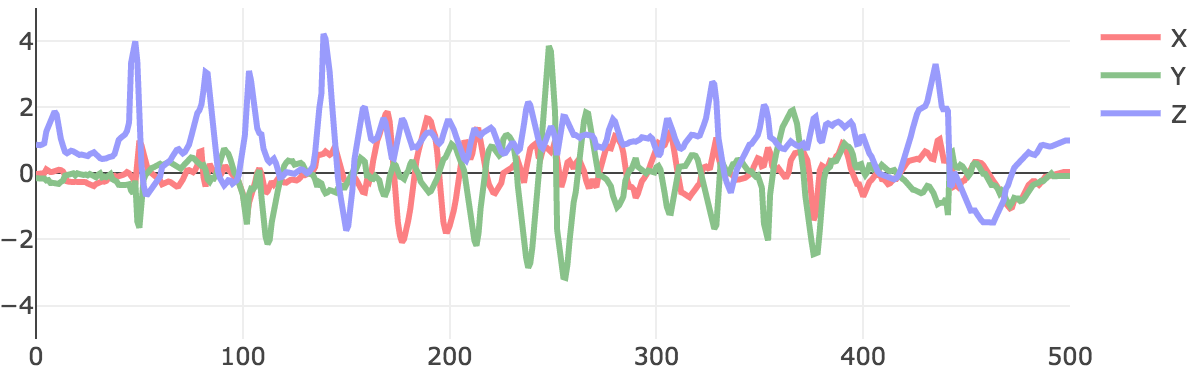
\includegraphics[width=15cm,keepaspectratio]{line_chart_2}
    \caption{line chart used to visualize sensor data in 2D and provide an interactive way to analyze the data}
    \label{fig:plotlylinechart}
\end{figure}

In GRAMOC the Plotly line chart was configured to hold three traces, one for each axis as shown in figure \vref{fig:plotlylinechart}. The main focus of the Plotly library is to give the user a convenient way to create interactive charts and not to provide high performance real-time charts. These aspects fit best into the archive page of GRAMOC, where the source of the data are static files and not real-time streams of data.

\section{D3.js}
The name \textit{D3} is an abbreviation of Data-Driven Documents, thats a very precise description of what this framework has to offer, namely the manipulation of documents based on data. The goal of D3.js is not to visualize data on documents and at the same time be able to handle all the things around the objects as well as implementing every imaginable feature, it is build to be perfect at one thing: ``efficient manipulation of documents based on data'', as stated on their website \autocite{d3}. Since one of the key features of GRAMOC is real-time representation of the data that is provided by a sensor, this framework was chosen to be used within the real-time display. D3.js has advantages as well as a few disadvantages. Probably the biggest advantage is that this framework is very lightweight. This means there is only a minimal overhead and therefore it is very fast compared to other frameworks or libraries like Plotly (see section \vref{sec:Plotly}). A disadvantage of D3.js would definitely be the lack of convenient high-level functions to create or modify objects. This lack of high-level functions leads to bigger development cost, because to implement simple feature it is necessary to write a lot of code compared to high-level solutions. In most high-level frameworks a developer just needs to call one function to create a chart and another one to add data to it. High-level functions are great to begin with, but to squeeze every last bit of performance out of the code, low-level functions are much better. Also to understand what is happening behind the code, low-level functions would be superior, because the developer has to do nearly every step on his own and not just call a magic function that does a lot of processing on its own. Therefore the lack of high-level functions could be seen as an advantage, because programmers that use low-level functions instead of high-level functions often have more knowledge about how the system works and thats clearly a good thing.

\subsection{Line Chart}
\label{subsec:d3linechart}
In GRAMOC D3.js was used to create a simple line chart to be able to visualize scientific sensor data in real-time. The chart is based on the line chart provided by Plotly, but with the distinction that the D3.js chart can render the given data faster, and therefore sustain the real-time support of the application. The design should be similar to the Plotly line chart to maintain a uniform design within the application. The chart with example data is shown below in figure \vref{fig:d3linechart}.

\begin{figure}[H]
    \centering
    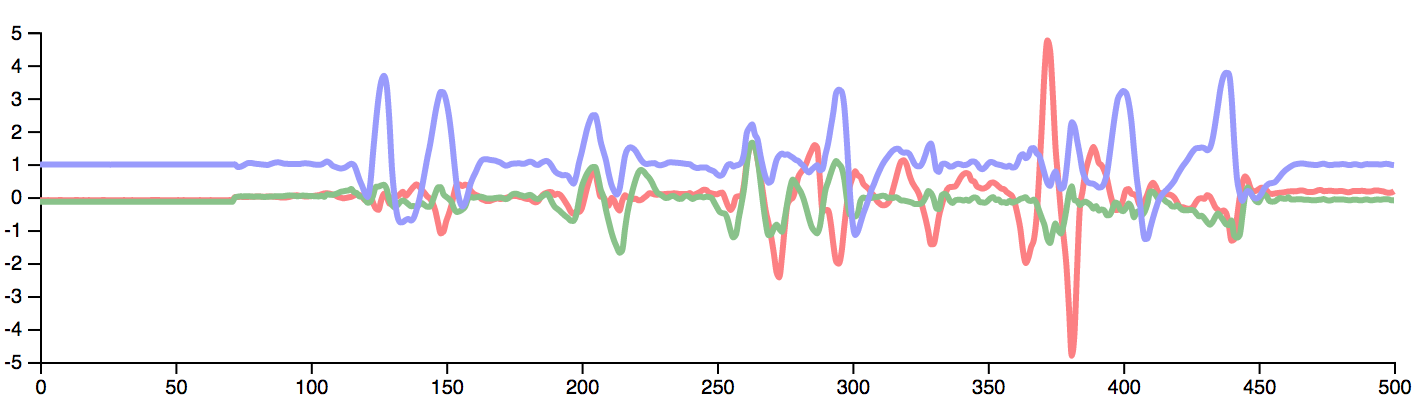
\includegraphics[width=15cm,keepaspectratio]{d3_line_chart}
    \caption{line chart used to visualize sensor data in 2D and be able to render in real-time}
    \label{fig:d3linechart}
\end{figure}

\section{Implementation}
As shown in figure \vref{fig:webserver-program-flow} the server asynchronously tries to connect with the UDP socket and starts listening for incoming connections on a specified port. The server keeps retrying to connect to the UDP socket until a connection is established. Without this connection no live data from the sensor can be forwarded to the web application. If a client connects on the before specified port the connection will be immediately upgraded to a socket connection and the web application will be served to the user. When the Webapp launches it will display the Home page, then the user can navigate to the 2D, the Archive or the About page, through the navigation bar at the top.

\subsection{2D Page}
If the user navigates to the 2D page, a line chart created with D3.js will be loaded. This chart consists of 3 traces, one for each axis of the sensor. The second chart displayed is a density chart created with HTML5 Canvas. This chart is represented by an ellipse, which is bent or stretched according to the received sensor data. Both these charts will be initialized and then the client emits a message to the server to start receiving the sensor data. This data will be used to update the charts accordingly. This page is responsible for visualizing the sensor data in real time and therefore its components are optimized to provide the necessary performance. The exact procedure is shown in figure \vref{fig:2d-page-flow}.

\begin{figure}[H]
    \centering
    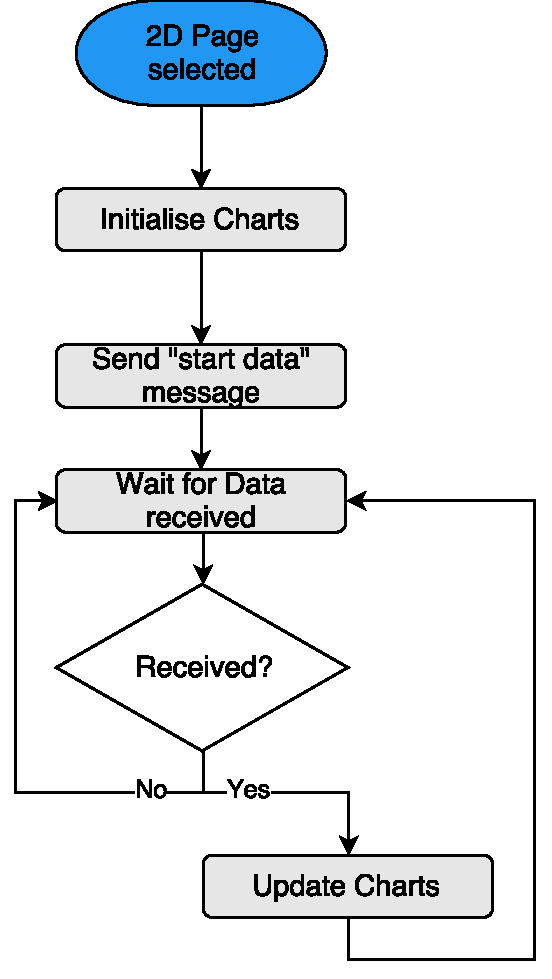
\includegraphics[width=5cm,keepaspectratio]{2d_page_flow}
    \caption{Flowchart of the procedure when 2D page is selected}
    \label{fig:2d-page-flow}
\end{figure}

\subsection{Archive Page}
The Archive page displays a line chart similar to the line chart on the 2D page, but with the focus on convenience rather than real-time performance. Therefore, Plotly is chosen to be used within this component. Along with the chart, a form will be available which is responsible to request the already recorded sensor data selected by the user. The execution flow of this component is depicted in figure \vref{fig:archive-page-flow}.

\begin{figure}[h]
    \centering
    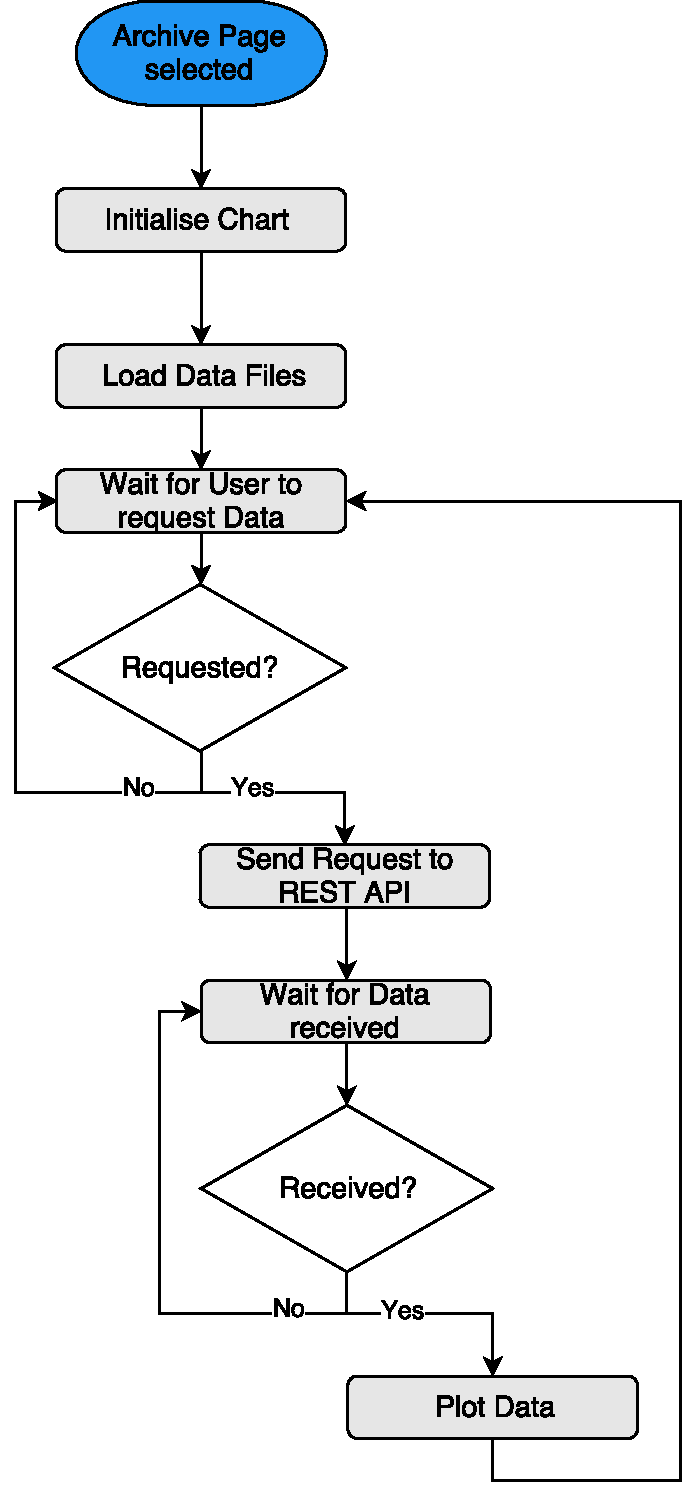
\includegraphics[width=7cm,keepaspectratio]{archive_page_flow}
    \caption{Flowchart of the procedure when Archive page is selected}
    \label{fig:archive-page-flow}
\end{figure}

\subsection{About Page}
The About page is simply a static page that displays a few informations about the project.

\begin{figure}[h]
    \centering
    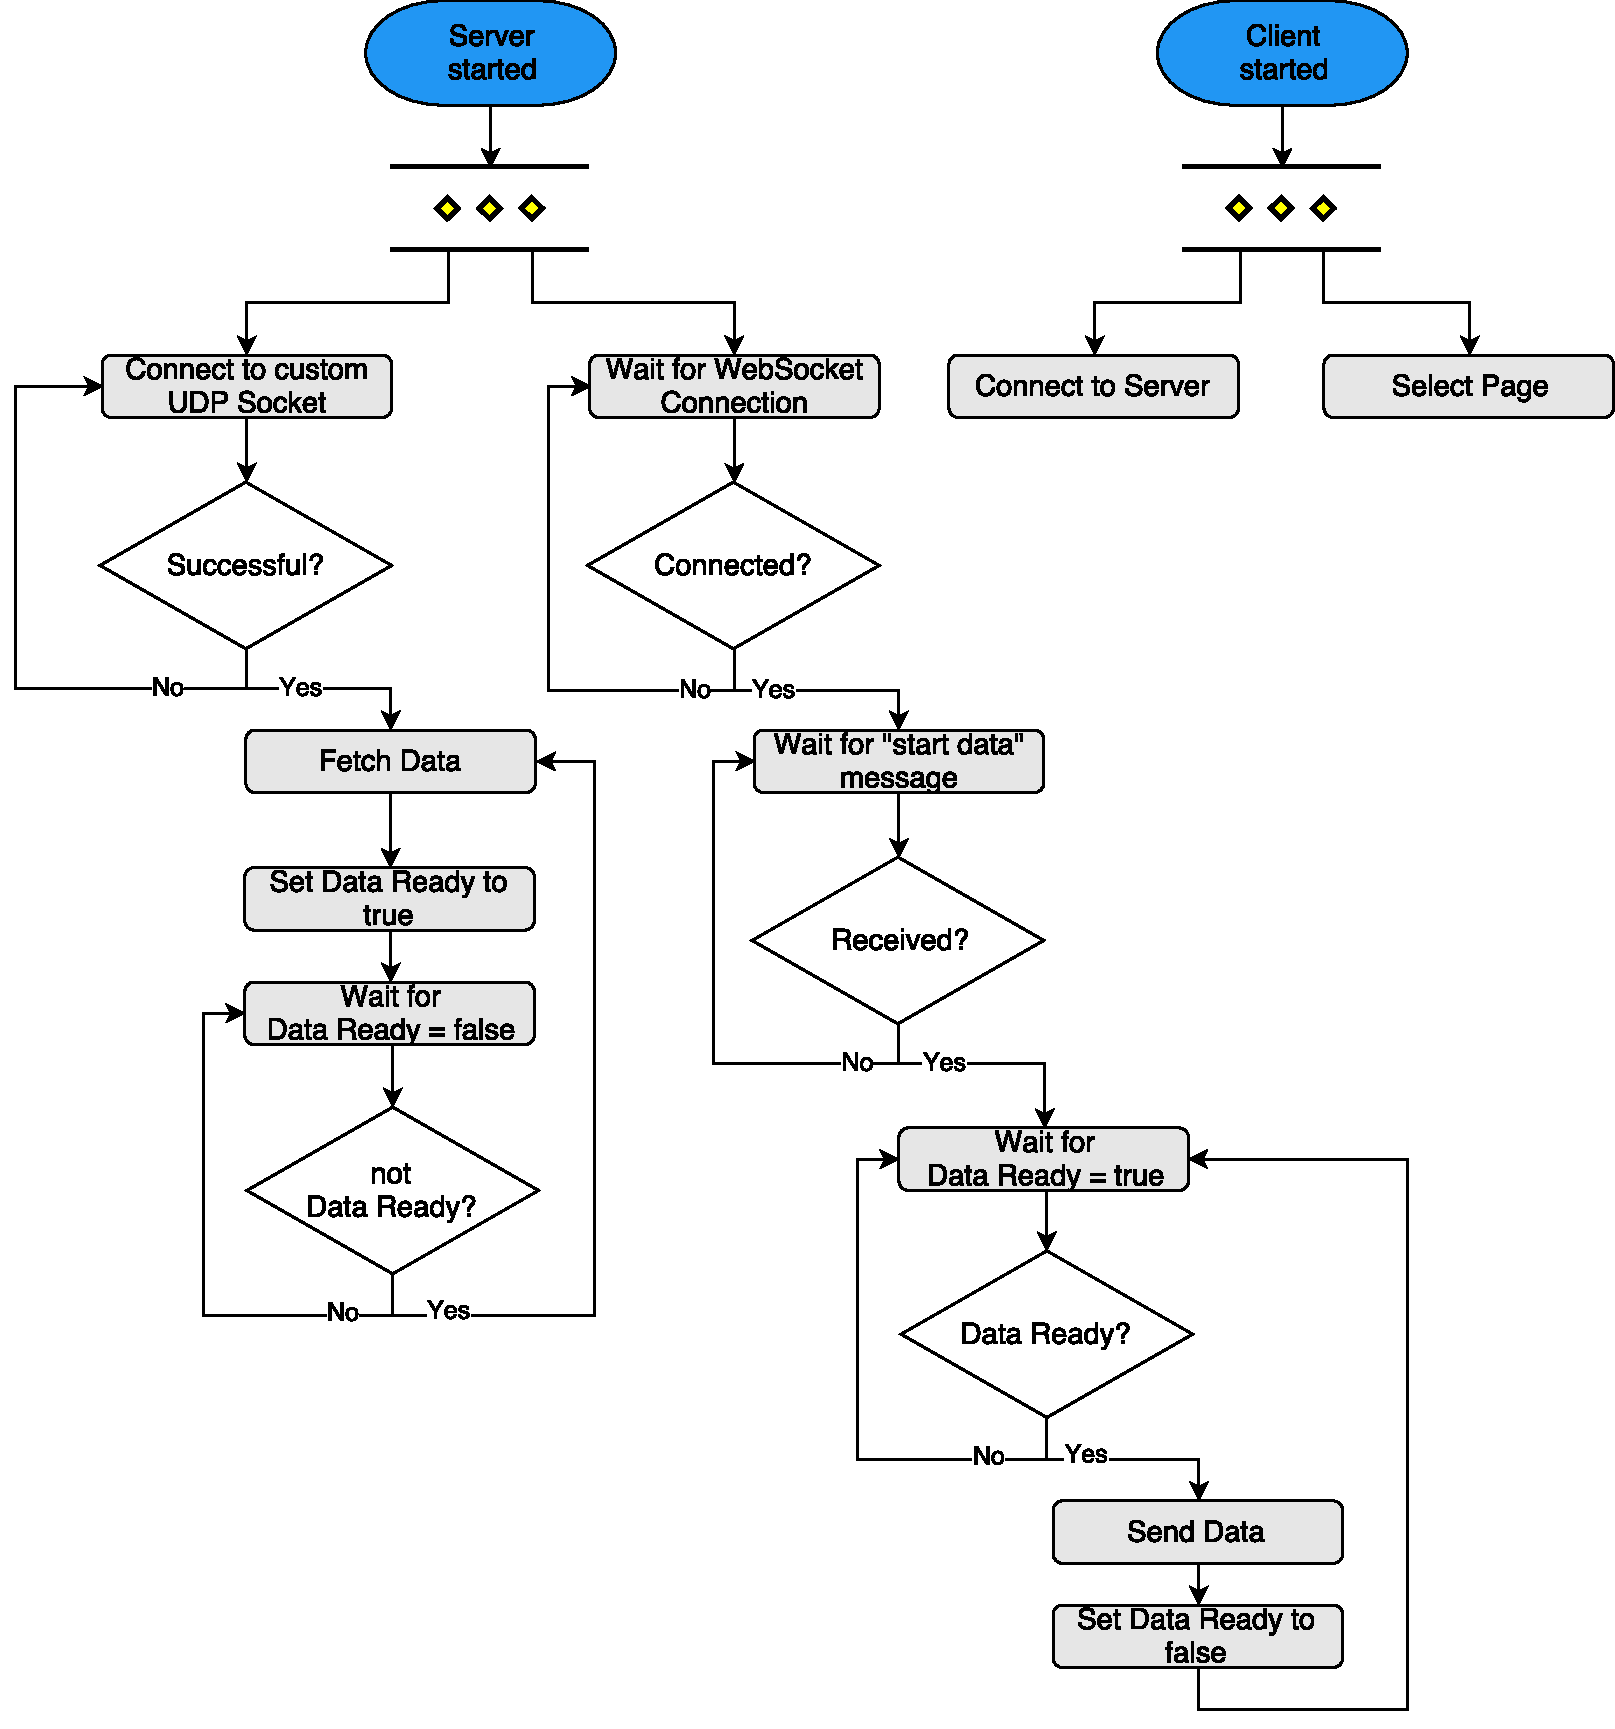
\includegraphics[width=15cm,keepaspectratio]{node_server_flow}
    \caption{Flowchart of web server and client program showing the procedure}
    \label{fig:webserver-program-flow}
\end{figure}

\chapter{Data Analysis}
\label{ch:dataanalysis}

\author{Nico Kratky}
%
\section {Regression Analysis}

Regression analysis is a statistical method to determine relationships between a response variable $ y $ and one or more predictor variables $ x_i $, where $ i = 1, 2, ..., p $. Linear regression analysis assumes that these predictor variables are related linear to the response variable.

\subsection{Simple Linear Regression}
\label{sec:slr}

Simple Linear Regression is a regression model that can only build a relationship between one predictor variable and one response variable. To find the best fit for this linear model the \textit{Ordinary Least Squares} method is used. The linear regression model builds a linear function

\begin{equation}
\label{eq:line}
    y = k * x + d
\end{equation}

that represents the predicted values. This function can also be denoted as

\begin{equation}
\label{eq:slr}
    y = \beta_0 + \beta_1 * x,
\end{equation}

where $ \beta_0 $ is the intercept and $ \beta_1 $ is the slope of the line.

The two regression parameters,

\begin{equation}
    \beta_1 = \frac{\sum_{i=1}^{n} (x_i - \bar{x}) * (y_i - \bar{y}))}{\sum_{i=1}^{n} (x_i - \bar{x})^2}
\end{equation}

\begin{equation}
    \beta_0 = \bar{y} - \beta_1 * \bar{x},
\end{equation}

that are used in this regression model are calculated using the least squares method. This method tries to minimize the sum of squared residuals.

\subsubsection{Example}

A good example for linear regression analysis is the ringsize of women. This example was taken from the website \url{http://www.crashkurs-statistik.de} \autocite{CrashkursSLR} \autocite{CrashkursMLR}.

If somebody wants to know the ringsize of his girlfriend, but does not want to ask her, it is possible to predict the size. To be able to do this a data basis has to be formed. A decisive factor for someones ringsize is for example the body height.

The data, which is depicted in table \vref{tab:slr_ringsize} can be used to calculate the regression coefficients using the formulae discussed in section \vref{sec:slr}. These calculations result in the two regression coefficients

\begin{equation}
    \beta_1 = \frac{\sum_{i=1}^{n} (x_i - \bar{x}) * (y_i - \bar{y}))}{\sum_{i=1}^{n} (x_i - \bar{x})^2} = 0.2838
\end{equation}

\begin{equation}
    \beta_0 = \bar{y} - \beta_1 * \bar{x} = 2.8457,
\end{equation}

which are slope and intercept, respectively.

\begin{table}[h]
    \centering
    \begin{tabular}{|l|l|l|l|l|l|l|l|l|l|l|}
    \hline
    \textbf{Person $ i $}    & \textbf{1} & \textbf{2} & \textbf{3} & \textbf{4} & \textbf{5} & \textbf{6} & \textbf{7} & \textbf{8} & \textbf{9} & \textbf{10} \\ \hline
    \textbf{Ringsize $ y $}  & 47.1       & 46.8       & 49.3       & 53.2       & 47.7       & 49.0       & 50.6       & 47.1       & 51.7       & 47.8        \\ \hline
    \textbf{Height $ x $}    & 156.3      & 158.9      & 160.8      & 179.6      & 156.6      & 165.1      & 165.9      & 156.7      & 167.8      & 160.8       \\ \hline
    \end{tabular}
    \caption{Ringsizes of example persons and their body heights}
    \label{tab:slr_ringsize}
\end{table}

After these calculations, the regression line can be plotted as shown in figure \vref{fig:slr_ringsize}.

\begin{figure}[h]
\centering
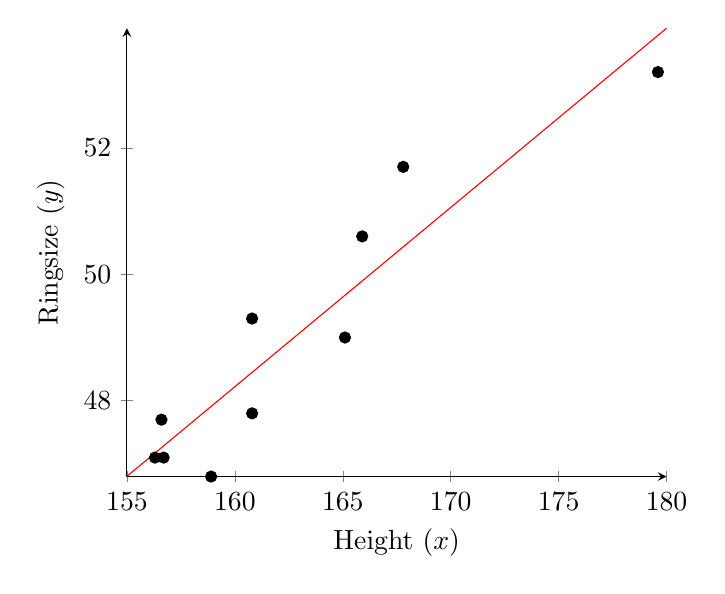
\begin{tikzpicture}
\begin{axis}[
    axis lines = left,
    xlabel = {Height ($x$)},
    ylabel = {Ringsize ($y$)},
]
\addplot [
    domain=155:180,
    color=red
]
{2.8457 + 0.2836 * x};

\addplot[
    only marks
]
table {
    x       y
    156.3   47.1
    158.9   46.8
    160.8   49.3
    179.6   53.2
    156.6   47.7
    165.1   49.0
    165.9   50.6
    156.7   47.1
    167.8   51.7
    160.8   47.8
};

\end{axis}
\end{tikzpicture}

\caption{Ringsizes of women. The single data points represents the gathered data. The red line depicts the regression line.}
\label{fig:slr_ringsize}
\end{figure}

To predict a persons ringsize, two options are available. The first option, which is not as accurate as the second one, is to simple read the predicted value from the regression line. If, for example, a person is 165cm tall, the proper ringsize would be a little bit less than 50. To be more precise, the second option can be used, which is to calculate the size using the regression coefficients. This can be done by applying the regression line to the height

\begin{equation}
    y = 2.8457 + 0.2836 * 165,
\end{equation}

which yields $ y = 49.64 $.

\subsection{Multiple Linear Regression}
\label{sec:mlr}

When the dependent variable depends on not just one variable, multiple linear regression analysis is used. This method uses two or more independent variables to describe the dependent variable. To calculate the regression coefficients the predictor variables have to be put into a $ n \times p $ matrix,

\begin{equation}
    X_{n,p} =
        \begin{bmatrix}
            1 & x_{1,1} & x_{1,2} & \cdots & x_{1,p} \\
            1 & x_{2,1} & x_{2,2} & \cdots & x_{2,p} \\
            1 & \vdots & \vdots & \ddots & \vdots \\
            1 & x_{n,1} & x_{n,2} & \cdots & x_{n,p}
        \end{bmatrix}
\end{equation}

where $ n $ is the amount of datasets and $ p $ is the amount of predictor variables $ + 1 $ because the intercept also has to be calculated. Also, a vector of all response variables

\begin{equation}
    y_{n} =
        \begin{bmatrix}
            y_{1} \\
            y_{2} \\
            \vdots \\
            y_{n}
        \end{bmatrix}
\end{equation}

has to be formed. These two matrices can be used to describe the basic multiple linear regression model

\begin{equation}
    \begin{bmatrix}
        y_{1} \\
        y_{2} \\
        \vdots \\
        y_{p}
    \end{bmatrix}
    =
    \begin{bmatrix}
            1 & x_{1,1} & x_{1,2} & \cdots & x_{1,p} \\
            1 & x_{2,1} & x_{2,2} & \cdots & x_{2,p} \\
            1 & \vdots & \vdots & \ddots & \vdots \\
            1 & x_{n,1} & x_{n,2} & \cdots & x_{n,p}
    \end{bmatrix}
    \begin{bmatrix}
        \beta_{0} \\
        \beta_{1} \\
        \vdots \\
        \beta_{p}
    \end{bmatrix},
\end{equation}

where $ \beta $ are the regression coeffecients. Or shorter

\begin{equation}
    y = X\beta.
\end{equation}

\todo{describe what leads to the formula below}

The problem with this equation is that it is possible that this equation does not have a solution. Therefore the $ y $ and $ X $ matrices are multiplied with the transpose of $ X $.

\begin{equation}
\label{eq:mlr}
    \hat{\beta} = (X^TX)^{-1} X^Ty
\end{equation}

\subsubsection{Example}

With this in mind, the example from section \vref{sec:slr} can be extended by more body parameters like weight and age, as they may also have an impact on the accuracy of the regression model. Figure \vref{tab:mlr_ringsize} depicts the ringsizes and body heights from the previous example, plus the weight and age of these people.

\begin{table}[H]
    \centering
    \begin{tabular}{|l|l|l|l|l|l|l|l|l|l|l|}
    \hline
    \textbf{Person $ i $}    & \textbf{1} & \textbf{2} & \textbf{3} & \textbf{4} & \textbf{5} & \textbf{6} & \textbf{7} & \textbf{8} & \textbf{9} & \textbf{10} \\ \hline
    \textbf{Ringsize $ y $}  & 47.1       & 46.8       & 49.3       & 53.2       & 47.7       & 49.0       & 50.6       & 47.1       & 51.7       & 47.8        \\ \hline
    \textbf{Height $ x_1 $}  & 156.3      & 158.9      & 160.8      & 179.6      & 156.6      & 165.1      & 165.9      & 156.7      & 167.8      & 160.8       \\ \hline
    \textbf{Weight $ x_2 $}  & 62         & 52         & 83         & 69         & 74         & 52         & 77         & 65         & 79         & 51          \\ \hline
    \textbf{Age $ x_3 $}     & 24         & 34         & 26         & 51         & 43         & 33         & 22         & 21         & 19         & 34          \\ \hline
    \end{tabular}
    \caption{Ringsizes of example persons and the appropriate body parameters}
    \label{tab:mlr_ringsize}
\end{table}

This dataset can now be used to form the previously explained matrices.

\begin{equation}
    X_{10, 3} =
    \begin{bmatrix}
        1 & 156.3 & 62 & 24 \\
        1 & 158.9 & 52 & 34 \\
        \vdots & \vdots & \vdots & \vdots \\
        1 & 160.8 & 51 & 34
    \end{bmatrix}
\end{equation}

\begin{equation}
    y_{10} =
    \begin{bmatrix}
        47.1 \\
        46.8 \\
        \vdots \\
        47.8
    \end{bmatrix}
\end{equation}

Using the regression parameter formula (see equation \vref{eq:mlr}) we get the regression parameters

\begin{equation}
    \hat{\beta} = (X^TX)^{-1} X^Ty =
    \begin{bmatrix}
        0.66 \\
        0.28 \\
        0.06 \\
        -0.02
    \end{bmatrix}.
\end{equation}

Using these parameters it is now possible to form the regression function

\begin{equation}
    y = 0.66 + 0.28 * x_1 + 0.06 * x_2 - 0.02 * x_3,
\end{equation}

which allows for data prediction.

In multiple linear regression analysis the predicted value can no longer be read off a graph, as the line is multi-dimensional. Lets assume that a woman is 170cm tall, weighs 68kg and is 29 years old. Inserting these values into the calculated model

\begin{equation}
    y = 0.66 + 0.28 * 170 + 0.06 * 68 - 0.02 * 29
\end{equation}

gives us the predicted ringsize $ y = 51.76 $.

\subsection{Working with Streaming Data}

As GRAMOC uses streaming data a few adjustements had to be made. The ordinary multiple linear regression model assumes that all observations are available when calculating the regression coefficients. Therefore a way of calculating these regression coefficients in a streaming way had to be found. To accomplish this the regression parameters have to be calculated incrementally. This means that the two parts of the regression parameter calculation, $ X^T X $ and $ X^T y $ have to be recalculated every time a new observation is made. These two matrices are then added up, since matrix addition between two $ n \times n$ matrices also result in a $ n \times n$ matrix. The sum of these matrices are named $ M $ and $ V $. This is possible as $ X^T X $ always returns a $ p \times p $ matrix and $ X^T y $ always returns a $ p $-dimensional vector.

When the regression coefficients are calculated,

\begin{equation}
    \hat{\beta_k} = (M + {X_k}^T X_k)^{-1}(V + {X_k}^T y_k),
\end{equation}

the sum of previous observation data is added to the current data, and then the procedure described in \vref{sec:mlr} can be applied.

This procedure was introduced in a regression calculation programm called StreamFitter, which also works with streaming data \autocite{StreamFitter}.

\subsection{$ r^2 $ - Coefficient of Determination}

$ r^2 $ is the quotient of the explained variation

\begin{equation}
    ESS = \sum_{i=1}^{n} (\hat{y}_i - \bar{y})^2
\end{equation}

and the total variation

\begin{equation}
    TSS = \sum_{i=1}^{n} (y_i - \bar{y})^2,
\end{equation}

\begin{equation}
    r^2 = \frac{ESS}{TSS}
\end{equation}

It is a measure for how much variation of the data can be explained with this regression model. $ r^2 $ values are ranged between $ 0 $ and $ 1 $, where $ 1 $ is considered a perfect fit and $ 0 $ says that no data can be explained using this regressino model.

\section{Implementation}



%Literaturverzeichnis
\clearpage
\addcontentsline{toc}{chapter}{\bibname}

\printbibliography


%%%----------------------------------------------------------

%%%Messbox zur Druckkontrolle
\chapter*{Messbox zur Druckkontrolle}



\begin{center}
{\Large --- Druckgröße kontrollieren! ---}

\bigskip

\Messbox{100}{50} % Angabe der Breite/Hoehe in mm

\bigskip

{\Large --- Diese Seite nach dem Druck entfernen! ---}

\end{center}



\end{document}
